\documentclass[12pt,a4paper]{book}
\usepackage[utf8]{inputenc}
\usepackage[english]{babel}
\usepackage[left=2cm,right=2cm,top=2cm,bottom=2cm]{geometry}

\usepackage{amsmath}
\usepackage{amsfonts}
\usepackage{amssymb}

\usepackage{graphicx}				% import external graphics ( \includegraphics command)
\usepackage{wrapfig}					% allow text to wrap around figures ( \begin{wrapfigure} )
\usepackage{subcaption}			% allows subfigures within figures. Subfloats have their own caption, and an optional global caption.

\usepackage{parcolumns}

\usepackage{booktabs}				% professional tables

\usepackage[shortlabels]{enumitem}

\usepackage{siunitx}					% standard international system of units of measurement

\usepackage{varioref}				% verbose references package
\usepackage{hyperref}				% references and links package
\hypersetup{
%    bookmarks = true,         	% show bookmarks bar?
    unicode = false,          	% non-Latin characters in Acrobat’s bookmarks
    pdftoolbar = true,        	% show Acrobat’s toolbar?
    pdfmenubar = true,        	% show Acrobat’s menu?
    pdffitwindow = false,     	% window fit to page when opened
    pdfstartview = {FitH},    	% fits the width of the page to the window
    pdftitle   =								% title
    		{Photonic Artificial Neural Networks},
    pdfsubject = 							% subject of the document
    		{Application of integrated silicon photonics to artificial neural network design},
    pdfauthor  = {Davide Bazzanella},		% author
    pdfcreator = {Davide Bazzanella},  	% creator of the document
    pdfkeywords={integrated, photonic,		% list of keywords
    							microring, resonator,		%
    							neural, network,					%
    							feedforward,							%
    							perceptron}, 						%
    pdfnewwindow = true,	% links in new PDF window
    colorlinks = true,		% false: boxed links; true: colored links
    linkcolor = black,		% color of internal links (change box color with linkbordercolor)
    citecolor = black,		% color of links to bibliography
    filecolor = black,		% color of file links
    urlcolor  = gray			% color of external links
}
\usepackage[noabbrev]{cleveref}		% clever references package

\usepackage{caption}			% Nice captions
\captionsetup{
		format			= hang,		% Indents the caption text, so it will ‘hang’ under the first line of the text.
		margin			= 25pt,		% width used for both, the left and right margin. Is equivalent to margin={25pt,25pt}
		font				= small,		% option affecting the whole caption (font).
		labelfont	= bf				% option affecting the caption label and separator (labelfont).
	 %textfont		=					% option affecting the caption text (textfont).
}

\usepackage{comment}			% multiline commenting \begin{comment}
\usepackage{cancel}			% package to cancel obliquely symbols

\usepackage{dsfont}			% generate correct 1-bold (identity operator) font
\usepackage{bm}					% generate correct bold greek letters
\usepackage{esint}				% to produce stroked integral \fint

\usepackage{tcolorbox}		% better boxes (also multiple equations)
\tcbuselibrary{theorems}

\usepackage{authblk}			% author managing package

\title{%
%	Photonic Artificial Neural Networks:\\
	Photonic Artificial Neuromorphic Networks:\\
%	Photonic Neuromorphic Networks:\\
%	Neuromorphic Photonics:\\
	\large All-Optical Activation Function%
	}
\author[]{Davide Bazzanella}
\affil[]{Department of Physics, University of Trento}

\usepackage[style=ieee]{biblatex}
\addbibresource{bib_articles.bib}
\addbibresource{bib_books.bib}
\addbibresource{bib_websites.bib}
\usepackage{csquotes}		% required by biblatex ???

\usepackage{makeidx}			% to create an index with terms and the corresponding page(s)
\makeindex

\usepackage[printonlyused]{acronym}
\usepackage{multicol}

\usepackage{tikz}							% externalize tikz images
\usepackage{pgfplots} 					% create plots with pgf/tikz
\pgfplotsset{compat=1.14} 			% README here http://pgfplots.sourceforge.net/pgfplots.pdf
	%\usepgfplotslibrary{external}
	\usetikzlibrary{external}			%
	\tikzexternalize								% activate!
	\tikzsetexternalprefix{tikz/}	% set subfolder
	%\tikzexternalize[prefix=tikz/] % activate!

\usepgfplotslibrary{fillbetween,dateplot} % need this to fill between functions
\usetikzlibrary{	patterns, decorations, decorations.markings, decorations.pathreplacing,
								shapes, shapes.geometric, shapes.misc, arrows, arrows.meta,
								positioning, intersections
								}

% USER DEFINED COMMANDS %
% define the symbols := and =: for ease of use
\usepackage{mathtools}
\newcommand{\defeq}{\vcentcolon=}
\newcommand{\eqdef}{=\vcentcolon}

\begin{document}
% define Capitalized names for chapter/section/...
\def\chapterautorefname{Chapter}
\def\sectionautorefname{Section}
\def\subsectionautorefname{Subsection}

\sisetup{separate-uncertainty = true}

% define the box around functions
\newtcolorbox{mymathbox}[1][]{colback=white, sharp corners, #1}

%\pagenumbering{alph}
%\maketitle
\frontmatter
\thispagestyle{empty}
\begin{titlepage}
\begin{center}


\includegraphics[width=0.7\textwidth]{figures/unitn_logo}
\vspace{3em}

\hrule
\vspace{2em}
{\LARGE \textsc{Department of Physics} \\}
\vspace{1em}
{\LARGE \textsc{Master Degree in Physics} \\}
\vfill
{ \huge %\bfseries
%	Photonic Artificial Neural Networks:\\
	Optical Bistability As Neural Network\\
	\vspace{0.5em}
	\huge %\bfseries
%	All-Optical Activation Function
	Nonlinear Activation Function
}
\vfill

% ATTENZIONE! Ha bisogno del pacchetto parcolumns per funzionare
\begin{parcolumns}{2}
   \colchunk   {	\Large Supervisor:\\
%   							\LARGE \textbf{Paolo Bettotti}\\
   							\LARGE Dr. Paolo Bettotti\\
   							\vspace*{1em}
   							\Large Co-supervisor:\\
%   							\LARGE \textbf{Enver Sangineto}
   							\LARGE Dr. Enver Sangineto
   							}
   \colchunk[2]{	\Large Graduant:\\
%   							\LARGE \textbf{Davide Bazzanella}
   							\LARGE Davide Bazzanella
   							}
\end{parcolumns}

\vspace*{3em}
\large 20$^\text{th}$ March 2018\\[0.1cm]
\hrule

\end{center}
\end{titlepage}
\thispagestyle{empty}

\cleardoublepage
%\pagenumbering{roman}
\tableofcontents

% Index
\cleardoublepage
%\addcontentsline{toc}{chapter}{Symbols and Acronyms}
%\printindex
%\markboth{INDEX}{}
\chapter*{Acronyms}
%\markboth{ACRONYMS}{}
\markboth{}{}
\begin{multicols}{2}
\begin{acronym}[EYDFA]
%	\acrodefplural{BUT}{Blocks Under Test}%
	
	\acro{AI}[AI]{Artificial Intelligence}
	\acro{ADF}[ADF]{All-Drop Filter}
	\acro{ANN}[ANN]{Artificial Neural Network}
	\acro{APF}[APF]{All-Pass Filter}
	\acro{AWG}[AWG]{Array Waveguide Grating}
	\acro{CMOS}[CMOS]{Complementary Metal-Oxide-Semiconductor}
	\acro{CPU}[CPU]{Central Processing Unit}
	\acro{CEL}[CEL]{Cross-Entropy Loss}
	\acro{DOF}[DOF]{Degree Of Freedom}
	\acro{EM}[EM]{Electro-Magnetic}
	\acro{EYDFA}[EYDFA]{Erbium-Ytterbiym-Doped Fiber Amplifier}
	\acro{FCA}[FCA]{Free Carrier Absorption}
	\acro{FCD}[FCD]{Free Carrier Dispersion}
	\acro{FEM}[FEM]{Finite Element Method}
	\acro{FSR}[FSR]{Free Spectral Range}
	\acro{FWHM}[FWHM]{Full-Width-Half-Maximum}
	\acro{GPU}[GPU]{Graphic Processing Unit}
	\acro{GVD}[GVD]{Group Velocity Dispersion}
	\acro{HBP}[HBP]{Human Brain Project}
	\acro{ICT}[ICT]{Information and Communication Technology}
	\acro{MAC}[MAC]{Multiply-and-Accumulate}
	\acro{MLP}[MLP]{Multi-Layer Perceptron}
	\acro{MSE}[MSE]{Mean-Square Error}
	\acro{MZI}[MZI]{Mach-Zehnder Interferometer}
	\acro{OSA}[OSA]{Optical Spectrum Analyzer}
	\acro{PIC}[PIC]{Photonics Integrated Circuit}
	\acro{ReLU}[ReLU]{Rectified Linear Unit}
	\acro{RC}[RC]{Reservoir Computing}
	\acro{RNN}[RNN]{Recurrent Neural Network}
	\acro{SGD}[SGD]{Stochastic Gradiend Descent}
	\acro{SOI}[SOI]{Silicon-on-Insulator}
	\acro{TE}[TE]{Tranverse Electric}
	\acro{TEM}[TEM]{Transverse Electro-Magnetic}
	\acro{TIR}[TIR]{Total Internal Reflection}
	\acro{TM}[TM]{Tranverse Magnetic}
	\acro{TOC}[TOC]{Thermo-Optic Coefficient}
	\acro{TOE}[TOE]{Thermo-Optic Effect}
	\acro{TPA}[TPA]{Two Photon Absorption}
	\acro{XOR}[XOR]{exclusive-or}
	\acro{VOA}[VOA]{Variable Optical Attenuator}
	\acro{WG}[WG]{waveguide}
\end{acronym}
\end{multicols}

\cleardoublepage
\pagenumbering{arabic}
\mainmatter
% introductory chapter ~ 5pg
\chapter*{Introduction}
\markboth{INTRODUCTION}{}
\addcontentsline{toc}{chapter}{Introduction}

\paragraph{The research field\\}
Research in the field of artificial neural networks has became more and more popular in the last few decades as the computing power available to the average institution increased further.
As a matter of fact, in the last two decades the calculation power which once belonged only to bulky, power hungry, and very expensive supercomputers, gradually became possible also for relatively more compact, efficient, and definitely cheaper servers and workstations.

This trend is dictated by the fact that artificial neural networks are usually simulated on conventional computers, which are on the other hand based on the von Neumann, or Princeton, architecture.
Implementations of this general purpose architecture are able to do any logical computation with a series of instructions.
However the downside of this suitability to generic computations is that it is often difficult to parallelize single operations and therefore certain tasks are inherently inefficient, both in energy and in time.
Moreover another problem is that it requires explicit programming for each singular task

The formalization of the von Neumann architecture dates back to 1945 and is as old as the first attempt in artificial neural networks.
Shortly after, research and industry efforts focused only on the development of the Princeton architecture, choosing it de facto as the primary design for computing devices.

In the recent years, help came from acceleration units known as Graphic Processing Units (GPU), which were developed for a completely different objective.
These GPUs, which are nowadays being designed specifically to accelerate calculations of artificial neural network simulations, are able to carry out a restricted set of instruction compared to CPUs, but are much more efficient both in power and in time, because of their parallel execution.

\paragraph{Todays software implementations\\}
Between the most famous examples of simulated neural network there certainly are the older Watson supercomputer from IBM and the more recent AlphaGo artificial intelligence.
Both of them arose to popularity because they defeated us humans to our own games.
Specifically the effort of Watson was aimed at prevailing the most strongest human contestants at \textit{Jeopardy!}, an American television game, and succeeded in 2011.
Watson was powered by a IBM supercomputer and used \SI{0.22}{\MW} of power.
AlphaGO, nevertheless, is a deep neural network that in 2016, through reinforced learning algorithms, defeated Lee Sedol, considered the most formidable master of Go, a complicated board game.

Another interesting case is given by SpiNNaker, of the University of Manchester.
It is composed by $10^4$ neurons connected by more that $10^7$ synapses, and is simulated on over 65 thousand 18-core ARM processors connected together.
Unlike the other two, its main goals are to simulate several neural mechanisms, such as the
operation of visual cortex.

Similarly to SpiNNaker, another effort in gaining better understanding of the human brain is \textit{The Blue Brain Project}, which is leaded by École Polytechnique Fédérale de Lausanne in collaboration with over one hundred other international research institutions and it is funded by the European Union.
This project is simulated on IBM Blue Gene supercomputers, each fitted with more than 100 thousand processors and consuming several \si{\MW} of power.

\paragraph{Present objectives and future trends\\}
We can distinguish two principal objectives in this research field.
The first one is a technological objective and is that of developing a more powerful computational instrument.
The second objective is instead a topic of more fundamental research: to use the tools of artificial neural networks to better understand biological neural networks such as our brain.

If the comprehension of the complex mechanism at the base of our brain has always been a very arduous assignment, the tasks that artificial neural network are facing become increasingly difficult while time passes.
Whereas in the past years public and private research groups trained themselves with "easier" problems, such as television or board games, today they are concentrating their efforts on more challenging goals.
Probably the most clear example of this tendency is given by the research on autonomous driving, where artificial neural networks are used primarily for real-time processing of data from several sensors..

A great number of businesses formed in recent years around these problems and many other will probably do the same for similar areas.
It is very likely that to achieve their objectives, even more powerful and complex artificial networks will be required.
Therefore more processors will be developed and put together to achieve impressive computing power.
However, one cannot expect to increase indefinitely the power, without significant improvements in efficiency.
Hence alternatives are sought.

\paragraph{Overview of current alternatives to simulations\\}

Apart from the vast majority of the research on neural networks, which is being carried out with simulations on powerful processors, a smaller portion of research is focused on building neural network physically.
Great efforts are made nowadays by many research institutions and companies to develop original computing architectures that allow artificial neural networks to run physically, instead of being simulated on conventional computers.

The reason why considerable improvements can be expected is that the path of designing hardware devices ad hoc for neural network computation has not yet been covered comprehensively.
Majors performance or efficiency enhancements are coming from the fact that those new architectures are conceived with parallel execution of specific operations in mind.
However, being designed for precise tasks makes them unsuitable for generic computation, which could in principle make them less easy to modify when needed, unlike simulations on conventional computers.

Many of these use the electronics framework, mainly because of the many benefits of the mature silicon technology and its CMOS-compatible production chain.
Specifically footprint and efficiency of CMOS devices has not yet stopped to grow since its discovery, in the past century.
However, a relatively small portion of these works also inquired simpler network fabrication with organic electronic materials, achieving remarkable results.

Among the most interesting projects which uses electronics there are TrueNorth of IBM and Neurogrid of Stanford University.
The former is part of a long-term research project funded by DARPA and has the aim of building an artificial neural network with the capabilities of brains of small mammalians, such as cats or mice.
In 2014 IBM showed a chip, named TrueNorth, containing 1 million artificial neurons and 256 millions synapses.
This network, relying on more than 5 billion transistors organized on an area of \SI{4.3}{\square\cm}, consumed only \SI{60}{\mW}.
The researcher also proved that connecting 48 of this chips together they obtained the equivalent of the brain of a mouse.

Similarly, the intention behind Neurogrid chip is to explore numerous hypothesis concerning mammalian brains, specifically about the inner mechanisms of operation of the cerebral cortex.
Stanford's implementation reaches the line of 1 million neurons, while only requiring \SI{5}{\W} of power consumption.
Moreover the communication lines between single neurons, the synapses, are provided by FPGAs and banks of SRAM.

Besides electronics, other kind of physical implementations are attempted from research teams.
Probably the most intriguing example is given by researches in photonics, which attempts to match electronics performance by overcoming its intrinsically weaknesses, such as power consumption.
Photonics has yet to reach achievements comparable to electronics, mainly due to the embryonic state of its technology.

\paragraph{My work\\}
My work has two related objectives.
The primary aim is to implement a proof of concept for a fundamental component of artificial neural networks: the neuron's activation function.
I plan to do so by employing the framework made available by integrated photonics.
The second intent is to bring together two until now distant fields of research: physics and information technology, specifically photonics and machine learning.
In fact generating knowledge transversal to the two research fields is at least as much important as the primary objective

The idea at the base of our physical implementation is to employ integrated devices already manufactured to create a proof of concept for the activation function.
The choice of integrated photonics is motivated by the fact that, unlike the electronic counterpart, does not suffer from the Joule effect.

Therefore in this work I will study a particular device, a microring resonator, and characterize its response to different inputs, for several working conditions.
This device can process information because it has, under certain circumstances, a nonlinear response function to its inputs.
Moreover, the same device might in principle be used in another important part of artificial neural network nodes: the weighted sum.
However, since this last point has already been discussed in literature and it requires less effort to produce acceptable results, it will not be at the center of this study.

%{WHAT AM I DOING\\why silicon photonics (CMOS compatibility)}
%The aim of this work is to put together two fields of research: physics and computer technology, specifically photonics and machine learning.
%The idea is to create a proof of concept for a physical implementation of a very important piece of any artificial networks, the activation function, by using integrated photonics as framework.
%Therefore I study a particular device, a microring resonator, and characterize its response to different inputs, for several working conditions.
%This device can process information because it has, under certain circumstances, a nonlinear response function to its inputs.

Moreover, the same device might in principle be used in another important part of artificial neural networks, the weighted sum.
However, since this last fact has already been discussed in literature and it requires less effort to produce acceptable results, it will not be at the center of this study.

%\paragraph{WHAT IMPROVEMENT WILL HAVE OVER EXISTING THINGS\\}
Since the aim is to create a proof of concept with structures not specifically designed, I don't expect extraordinary performance both in speed and in efficiency.
These aspects will be discussed in the conclusive words an will be studied to their fullest only in future works.
%This project is consistent with those efforts because it studies a novel hardware implementation for an activation function.
%Such implementation uses only optical phenomena and as such it is original.

%\paragraph{WHY AM I DOING THIS WORK (project BACKUP)\\}
Furthermore, regarding the second objective, my work is part of a bigger project, BACUKP, with a wider scope and a more ambitious goal.
It attempts to connect three fields of research, normally quite distant from each other: physics, computing technology, and biology.
The main idea is to use the integrated photonics framework (physics) to build an artificial neural network (computing technology) on chip, where one could grow and, at least partially control, real neurons (biology).
The aim is to develop a methodologies and devices that will allow us to study neural activity from a bottom-up perspective.

\paragraph{Structure of the thesis\\}

The first chapter of this thesis is intended as an introduction to the world of artificial neural networks.
After a brief historical summary, I describe the main aspects of neural networks and their working principles.
Then I focus on the description of the simplest type of artificial networks, the feedforward network, and finally and overview on other kind of networks.
Since the aim of this thesis is to tackle a specific problem, this chapter is not meant to be comprehensive foundation or compendium on the matter.
Later, the chapter is concluded with an introductory description of the language Python and the library PyTorch, used in this work for artificial network simulations.

The second chapter introduces the physics which I will study.
Again, after a short explanation on the basic devices used in the field, I will describe in depth the device studied for the task.
Having clarified the physics underneath, I ought to explain how I am going to use this physics to implement (part of) an artificial neural network.
I will address these topics both from the theoretical point of view and from the numerical one, with simulation of the specific (simplified) system.

The third chapter in dedicated to the description of the experimental work.
At the beginning the problem of the selection of the sample is discussed, along with the definition of the device chosen.
After, I characterize the different behaviors with detailed data.
Finally, an explanation on how the device will be used in the neural network viewpoint and the corresponding tests of operation.

% first chapter "Artificial Neural Networks" ~ 15pg
\chapter{Artificial Neural Networks}
\label{ch:Artificial_Neural_Networks}
%\section{Introduction}
%\label{sec:AAN_intro}
%A neural network is an interconnected assembly of simple processing elements, units or nodes, whose functionality is loosely based on the animal neuron. The processing ability of the network is stored in the interunit connection strengths, or weights, obtained by a process of adaptation to, or learning from, a set of training patterns.

\acfp{ANN} are computational systems which elaborate information in a way that is loosely inspired by the operation of biological neural networks (animal brains).
Biological networks are superior in performance to computers and extremely more efficient in difficult tasks such as classification (e.g. image recognition) and prediction (e.g. pattern recognition).
The underlying idea is to copy some of their mechanisms and exploit them for computational applications.
These systems are intrinsically parallel in operation, do not require specific programming to operate, and modify their behavior through a learning process to improve their accuracy in a certain task.

Mathematically speaking, \acsp{ANN} are a collection of nodes, each one of them elaborates the information and is somehow connected to the other.
Artificial networks can be either simulated on computers or physically built on hardware designed ad hoc.
At this time, \acsp{ANN} are mainly implemented by simulations, however the technological progress is withheld by limitation in computing power and efficiency.
Training a complex artificial neural network with computers at the state of art might take even weeks.
Thus, with the aim of improving performance from simulated networks, research on hardware architectures is surging: digital, analog, electrical, and optical devices are being developed.

\section{History}
\label{sec:History}
It is widely acknowledged that the opening work of this research field was made in 1943 by Warren McCulloch and Walter Pitts, a neurophysiologist and a mathematician respectively.
In their research work, they described the operating mechanism of biological neurons by modeling a simple electronic circuit \cite{McCulloch1943}.

The following important work was made by Donald O. Hebb, who hypothesized the neural plasticity in 1949 \cite{hebb1949organization}.
He pointed out the fact that neural pathways are strengthened each time they are used, a concept known as \textit{Hebbian learning}.

During the late 1950s and the early 1960s, as computers became more powerful, many promising works were published.
Some simulated operation of artificial networks on calculators, e.g. Farley and Clark \cite{Farley1954} and Rochester \cite{Rochester1956}.
Other produced circuitry that implemented on hardware such networks, e.g. Rosenblatt \cite{frank1957perceptron,Rosenblatt1958}.
However, despite the early successes of neural networks, the traditional computing architecture (von Neumann architecture) was chosen as the preferred computing architecture.
%As a result, funding and therefore also research diminished drastically in the following decades.

The reason why this happened, probably, was due to several concurring facts.
First of all, in the same time period (1969) a research paper by Minksi and Papert \cite{minski1969perceptrons}, which identified two important problems.
The basic perceptron was not able to execute the \ac{XOR} operation, unlike the logical circuits at the base of von Neumann architecture.
Moreover, the research stated the fact that more complex networks such as multiple- or deep-layered networks were not possible (at that time) because of the lack of adequate processing power.

%who discovered two key issues with the computational machines that processed neural networks.
%The first was that basic perceptrons were incapable of processing the exclusive-or circuit.
%The second was that computers didn't have enough processing power to effectively handle the work required by large neural networks.
%in the same time period a research paper wrongly suggested that there could not be any multiple-layered neural network.

In addition to this research, the early successes of some works on neural networks pointed to an overestimation of the artificial neural networks potential, also held back by the technological capacity of the time.
Finally, important questions of philosophical nature came to light, such as the fear fueled debate on the impact on our society of a class of computers able to think.
This very controversy, i.e. the \ac{AI} problem, is discussed still today \cite{stanford.edu}.

Sometime during the 1980s the interest for this computing method was reinvigorated.
The main stimulation was probably given by a number of works which suggested methods to implement multi-layered networks distributing pattern recognition errors through the all the layers in the network.
This method is now called \textit{backpropagation}.

In today's research and technology, artificial neural networks are used in numerous applications.
However, the development is made slowly, due to technological limitation in computational power of present processors.

\section{Basis of Neural Networks}
\label{sec:Basis_of_Neural_Networks}

A neural network is a collection of processing elements, or nodes, interconnected in an arbitrary topology.
From its input nodes, the network accepts information, which will propagate into the inner nodes through the interconnections and will get elaborated at each node.
At the end of the network, there will be a number of output nodes, with the task of reading a portion of the inner nodes.
The inner nodes are also called hidden, because they are not meant to be accessible to the external world.
A generic scheme of such network is shown in \autoref{fig:generic_NN} \vpageref{fig:generic_NN}.

\begin{figure}[ht]
	\centering
	\tikzsetnextfilename{GenericNN}
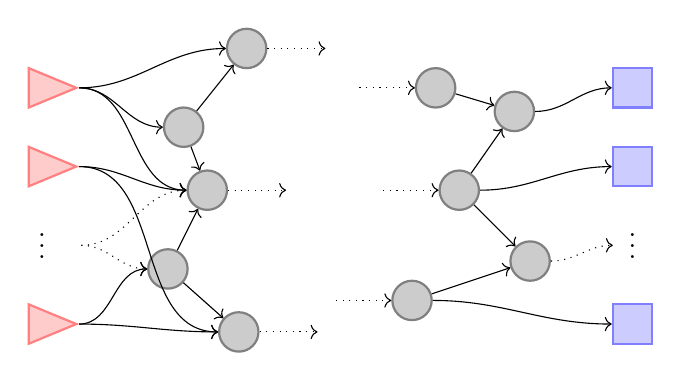
\begin{tikzpicture}
	[%
	input/.style ={isosceles triangle,	draw=red!50,		fill=red!20,		thick,	inner sep=0pt,	minimum size=5mm},%
	inner/.style ={circle,							draw=black!50,	fill=black!20,	thick,	inner sep=0pt,	minimum size=5mm},%
	output/.style={rectangle,					draw=blue!50,	fill=blue!20,	thick,	inner sep=0pt,	minimum size=5mm},%
	]

	% nodes
	\foreach \i in {0,1,3} \node (input\i) at (0,2.5-\i) [input] {};
	
	\node (inner0) at (1.6, 0.2) [inner] {};
	\node (inner1) at (1.8, 2.0) [inner] {};
	\node (inner2) at (2.1, 1.2) [inner] {};
	\node (inner3) at (2.5,-0.6) [inner] {};
	\node (inner4) at (2.6, 3.0) [inner] {};

	\node (inner5) at (4.7,-0.2) [inner] {};	
	\node (inner6) at (5.0, 2.5) [inner] {};
	\node (inner7) at (5.3, 1.2) [inner] {};
	\node (inner8) at (6.0, 2.2) [inner] {};
	\node (inner9) at (6.2, 0.3) [inner] {};	
	
	\foreach \i in {0,1,3} \node (output\i) at (7.5,2.5-\i) [output] {};
	
	% interconnections
	\draw [->] (input0) to [out=0,in=180] (inner1);	
	\draw [->] (input0) to [out=0,in=180] (inner2);	
	\draw [->] (input0) to [out=0,in=180] (inner4);	
	\draw [->] (input1) to [out=0,in=180] (inner2);	
	\draw [->] (input1) to [out=0,in=180] (inner3);	
	\draw [dotted, ->] (0.5,0.5)  to [out=0,in=180] (inner0);	
	\draw [dotted, ->] (0.5,0.5)  to [out=0,in=180] (inner2);	
	\draw [->] (input3) to [out=0,in=180] (inner0);	
	\draw [->] (input3) to [out=0,in=180] (inner3);	
	
	\draw [->] (inner0) to (inner3);
	\draw [->] (inner0) to (inner2);
	\draw [->] (inner1) to (inner2);
	\draw [->] (inner1) to (inner4);
	
	\draw [dotted, ->] (inner2) to +(0:1);
	\draw [dotted, ->] (inner3) to +(0:1);
	\draw [dotted, ->] (inner4) to +(0:1);
	
	\draw [dotted, <-] (inner5) to +(180:1);
	\draw [dotted, <-] (inner6) to +(180:1);
	\draw [dotted, <-] (inner7) to +(180:1);
	
	\draw [->] (inner5) to (inner9);	
	\draw [->] (inner6) to (inner8);
	\draw [->] (inner7) to (inner8);
	\draw [->] (inner7) to (inner9);
	
	\draw [->] (inner5) to [out=0,in=180] (output3);
	\draw [->] (inner7) to [out=0,in=180] (output1);
%	\draw [dotted,->] (inner7) to [out=0,in=180] (7.25,0.5);	
	\draw [->] (inner8) to [out=0,in=180] (output0);
%	\draw [->] (inner8) to [out=0,in=180] (output1);
	\draw [dotted,->] (inner9) to [out=0,in=180] (7.25,0.5);	
%	\draw [->] (inner9) to [out=0,in=180] (output3);
	
	\foreach \i in {0,7.5} \node at (\i,0.6) {$\vdots$};
	
\end{tikzpicture}
	\caption{	Generic scheme of a neural network. %
						Triangles (red) are input nodes, circles (grey) are inner nodes, and squares (blue) are output nodes. %
						Interconnections among nodes are represented by arrows: %
						continuous when both elements are drawn, and dotted otherwise.
						%						I chose a non-standard representation to emphasize the nonlinear nodes, which will use a nonlinear activation function. %
						}
	\label{fig:generic_NN}
\end{figure}

Nodes can all implement the same function or behave differntly, depending on the type of neural network.
%Each node can operate in the same way of the others or in a completely different manner, depending on the type of neural network.
The operation of nodes resembles that of animal neurons: various input gets collected and elaborated together to obtain an output, which will become one of the many inputs for subsequent neurons/nodes.
Specifically, the most used model for neurons is the McCulloch–Pitts (MCP) neuron.
It is divided into two parts, as shown in \autoref{fig:generic_node}: the first part is a weighted sum of the inputs, while the second part is given by the so called activation function.
\newpage
\begin{figure}[ht]
	\centering
	\tikzsetnextfilename{GenericNode}
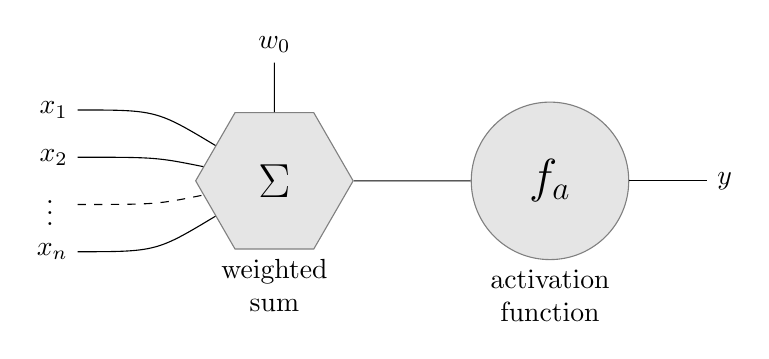
\begin{tikzpicture}
	\node [shape=circle, minimum size=2cm, draw=gray!100, fill=gray!20]%
				(af) at (1.5,0) {\LARGE $f_a$};
	\node at (af.south) [below, align=center] {activation \\ function};
	\node [regular polygon, regular polygon sides=6, minimum size=2cm, draw=gray!100, fill=gray!20]%
				(ws) at (-2,0) {\LARGE $\Sigma$};
	\node at (ws.south) [below, align=center] {weighted \\ sum};
	\draw (ws) to (af);
	\foreach \i in {1,2,4}	\draw (-4.5,1.5-0.6*\i) .. controls (-3.5,1.5-0.6*\i) .. (ws);
	\draw [dashed] (-4.5,-0.3) node {$\vdots\qquad$} .. controls (-3.5,-0.3) .. (ws);
	\foreach \i in {1,2}		\node at (-4.5,1.5-0.6*\i) [left] {$x_\i$};
	\node at (-4.5,-0.9)  [left] {$x_n$};
	\draw (-2,1.5) node [above] {$w_0$} to (ws);
	\draw (af) to (3.5,0) node [right] {$y$};
\end{tikzpicture}
	\caption{Generic node representation. $x$-values are inputs, $y$-values are outputs, $w_0$ is the bias.}
	\label{fig:generic_node}
\end{figure}
The node is described mathematically by \cref{eq:Generic_node_function}
\begin{equation}
y = f_a \left(  w_0 + \sum_{i=1}^{n} w_i x_i \right),
\label{eq:Generic_node_function}
\end{equation}
where $f_a$ is the activations function, evaluated on the sum of the input $x_i$ weighted with $w_i$, plus a bias $w_0$.

Each node accepts values at its inputs and produces an output accordingly.
However, in addition to the input, the output depends also on the node's parameters: the weights and the bias, which are usually changed outside the operative phase of the neural network (see \autoref{sec:Working_Principles_of_ANNs}).

Moreover it is mandatory for the activation function $f_a\left(\cdot\right)$ to be nonlinear, because otherwise a collection of nodes will result in just a weighted sum of its inputs.
Two examples of nonlinear function are shown below in \autoref{fig:activation_function_examples}.

\begin{figure}[ht]
	\begin{subfigure}[b]{0.49\textwidth}
		\centering
		\tikzsetexternalprefix{tikz/}	% set subfolder
\tikzsetnextfilename{HeavisideThetaFunction}
\begin{tikzpicture}[baseline]
	\begin{axis}[%
%			yticklabel pos=upper,%
			title ={$\Theta(x)$},%
			xlabel={$x$},%
%			ylabel={$\Theta(x)$},%
		]
		\newcommand\LIM{5}
		\addplot [blue, domain=-\LIM:0,	samples=501,]	{0};
		\addplot [blue, domain=0:\LIM,		samples=501,]	{1};
	\end{axis}
\end{tikzpicture}
		\caption{}
		\label{fig:activation_function_example_1}
  \end{subfigure}
  \begin{subfigure}[b]{0.49\textwidth}
  		\centering
		\tikzsetexternalprefix{tikz/}	% set subfolder
\tikzsetnextfilename{LogisticFunction}
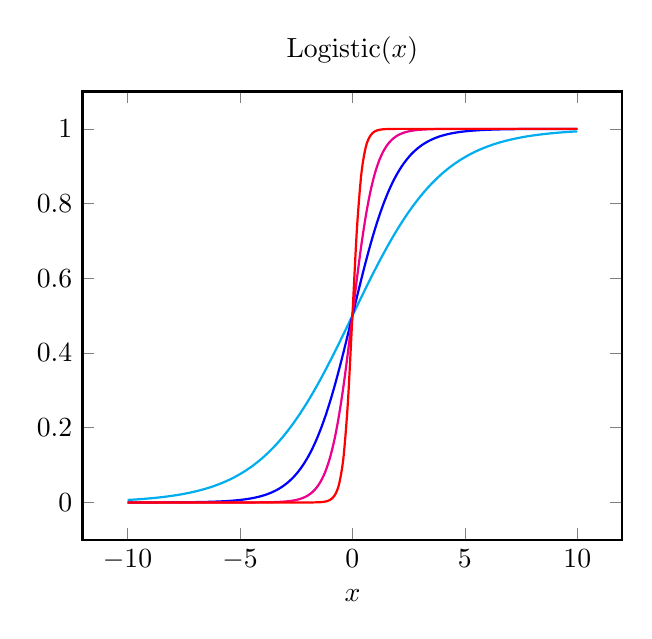
\begin{tikzpicture}[baseline]
	\begin{axis}[%
%			yticklabel pos=upper,%
			title ={$\mathrm{Logistic}(x)$},%
			xlabel={$x$},%
%			ylabel={$\mathrm{Logistic}(x)$},%
			thick,
			samples=101,
			smooth
		]
		\newcommand\LIM{10}
		\addplot [cyan, 		domain=-\LIM:\LIM]	{(1+exp(-0.5*x))^-1};
		\addplot [blue,	 	domain=-\LIM:\LIM]	{(1+exp(-1.0*x))^-1};
		\addplot [magenta,	domain=-\LIM:\LIM]	{(1+exp(-2.0*x))^-1};
		\addplot [red, 		domain=-\LIM:\LIM]	{(1+exp(-5.0*x))^-1};
	\end{axis}
\end{tikzpicture}
		\caption{}
		\label{fig:activation_function_example_2}
  \end{subfigure}
  \caption{Examples of activation function: (\ref{fig:activation_function_example_1}) is the well-known step function, or Heaviside $\Theta$, (\ref{fig:activation_function_example_2}) depicts a few functions from the family of the Logistic functions.}
  	\label{fig:activation_function_examples}
\end{figure}

One can distinguish at least three type of nodes in every neural network: input, inner/hidden, and output nodes.
Input nodes take one input value, from the outside of the neural network, and pass it on to the inner nodes unchanged.
Inner/hidden nodes take many inputs and generate an output through the activation function.
Output nodes, similarly to input nodes, take one input value, from the inside of the \acs{ANN}, and pass it on to the outside.

\subsection*{Standard Representation}
%This is not the orthodox description, but I claim that it is more consistent than the standard representation with the idea of functional \textit{black box}, in which input and output are the only visible nodes, while the other are hidden inside.
The way I depicted a generic neuromorphic network in \autoref{fig:generic_NN} is not the standard representation used in books and research papers.
The main difference is that usually weights are commonly represented on the connection between the nodes, which are then designated to apply only the activation function.
Moreover the input layer is linear as it feeds the inner nodes with the input data, while the output layer is actually given by the last nonlinear layer of the inner nodes.
A generic network is shown in \autoref{fig:standardNNdesc}.

\begin{figure}[ht]
	\begin{subfigure}[b]{0.49\textwidth}
		\centering
		\tikzsetnextfilename{standardNNdesc}
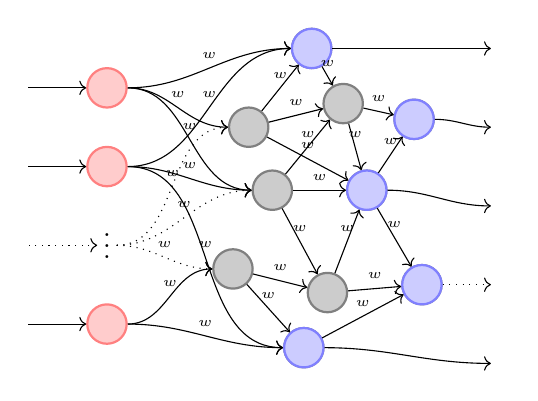
\begin{tikzpicture}
	[%
	input/.style ={circle,	draw=red!50,		fill=red!20,		thick,	inner sep=0pt,	minimum size=5mm},%
	inner/.style ={circle,	draw=black!50,	fill=black!20,	thick,	inner sep=0pt,	minimum size=5mm},%
	outer/.style ={circle,	draw=blue!50,	fill=blue!20,	thick,	inner sep=0pt,	minimum size=5mm},%
	]

	\newcommand\lin{0}
	\newcommand{\lout}{5}
	
	% nodes
	% input
	\foreach \i in {0,2,3} \node (input\i) at (\lin,0.5+\i) [input] {};
	\node (input1)		at (\lin,1.5) {}; 		\node at (\lin,1.6) {$\vdots$};
	% inner
	\foreach \n/\x/\y in {	0/1.6/1.2, 1/1.8/3.0, 2/2.1/2.2, 5/2.8/0.9, 6/3.0/3.3, %
												3/2.5/0.2, 4/2.6/4.0, 7/3.3/2.2, 8/3.9/3.1, 9/4.0/1.0 %
												}
			\node (inner\n) at (\x,\y) [inner] {};
	% outer
	\foreach \n/\x/\y in {	3/2.5/0.2, 4/2.6/4.0, 7/3.3/2.2, 8/3.9/3.1, 9/4.0/1.0 }
			\node (outer\n) at (\x,\y) [outer] {};
	% output
	\foreach \i in {0,1,2,3,4} \node (output\i) at (\lout,\i) {};
	
	% interconnections
	% to input
	\foreach \i/\type in {0/solid, 1/dotted, 2/solid, 3/solid}
		\draw [<-, \type] (input\i) -- ++(-1,0);
	
	% input to inner
	\foreach \i/\o in {0/0, 0/3, 2/2, 2/3, 2/4, 3/1, 3/2, 3/4}
		\draw [->] (input\i) to [out=0,in=180] node [midway, above] {\tiny{ $w$ } } (inner\o);
		
	\foreach \i/\o in {1/0, 1/1, 1/2}
		\draw [dotted, ->] (input\i) to [out=0,in=180] node [midway, above] {\tiny{ $w$ } } (inner\o);

	% inner to inner
%	\node at (0,0) {ciao};
	\foreach \i/\o in {	0/3, 0/5, 1/4, 1/6, 1/7, 2/5, 2/6, 2/7, %
											3/9, 4/6, 5/7, 5/9, 6/7, 6/8, 7/8, 7/9}
		\draw [->] (inner\i) -- (inner\o) node [midway, above] {\tiny{ $w$ } };
	
	% outer to output	
	\foreach \i/\o in {3/0, 7/2, 8/3, 4/4}
		\draw [->] (outer\i) to [out=0,in=180] (output\o);
				
	\foreach \i/\o in {9/1}
		\draw [dotted, ->] (outer\i) to [out=0,in=180] (output\o);
	
\end{tikzpicture}
		\caption{Standard way of representing networks}
		\label{fig:standardNNdesc}
  \end{subfigure}
  \begin{subfigure}[b]{0.49\textwidth}
  		\centering
		\tikzsetnextfilename{BlackBoxNN}
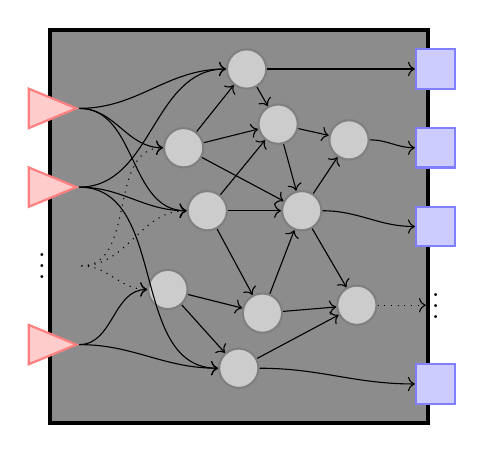
\begin{tikzpicture}
	[%
	input/.style ={isosceles triangle,	draw=red!50,		fill=red!20,		thick,	inner sep=0pt,	minimum size=5mm},%
	inner/.style ={circle,							draw=black!50,	fill=black!20,	thick,	inner sep=0pt,	minimum size=5mm},%
	output/.style={rectangle,					draw=blue!50,	fill=blue!20,	thick,	inner sep=0pt,	minimum size=5mm},%
	]

	\newcommand\lin{0}
	\newcommand{\lout}{5}
	
	% black box
	\filldraw [thick, draw=black, fill=gray!90, line width=0.5mm] (0.1,-1.5) rectangle (4.9,3.5);	
	
	% nodes
	\foreach \i in {0,1,3} \node (input\i) at (\lin,2.5-\i) [input] {};
	
	\foreach \i in {0,1,2,4} \node (output\i) at (\lout,3-\i) [output] {};
	
	\node (inner0) at (1.6, 0.2) [inner] {};
	\node (inner1) at (1.8, 2.0) [inner] {};
	\node (inner2) at (2.1, 1.2) [inner] {};
	\node (inner3) at (2.5,-0.8) [inner] {};
	\node (inner4) at (2.6, 3.0) [inner] {};

	\node (inner5) at (2.8,-0.1) [inner] {};
	\node (inner6) at (3.0, 2.3) [inner] {};
	\node (inner7) at (3.3, 1.2) [inner] {};
	\node (inner8) at (3.9, 2.1) [inner] {};
	\node (inner9) at (4.0, 0.0) [inner] {};
	
	\node (input2)		at (\lin,0.5) {}; 		\node at (\lin,0.6) {$\vdots$};
	\node (output3)	at (\lout,0.0) {}; 	\node at (\lout,0.1) {$\vdots$};
	
	% interconnections
	\draw [->] (input0) to [out=0,in=180] (inner1);
	\draw [->] (input0) to [out=0,in=180] (inner2);
	\draw [->] (input0) to [out=0,in=180] (inner4);
	\draw [->] (input1) to [out=0,in=180] (inner2);
	\draw [->] (input1) to [out=0,in=180] (inner3);
	\draw [->] (input1) to [out=0,in=180] (inner4);
	\draw [dotted, ->] (0.5,0.5)  to [out=0,in=180] (inner0);
	\draw [dotted, ->] (0.5,0.5)  to [out=0,in=180] (inner1);
	\draw [dotted, ->] (0.5,0.5)  to [out=0,in=180] (inner2);
	\draw [->] (input3) to [out=0,in=180] (inner0);
	\draw [->] (input3) to [out=0,in=180] (inner3);
	
	\draw [->] (inner0) to (inner3);
	\draw [->] (inner0) to (inner5);
	\draw [->] (inner1) to (inner4);
	\draw [->] (inner1) to (inner6);
	\draw [->] (inner1) to (inner7);
	\draw [->] (inner2) to (inner5);
	\draw [->] (inner2) to (inner6);
	\draw [->] (inner2) to (inner7);
	\draw [->] (inner3) to (inner9);
	\draw [->] (inner4) to (inner6);
	\draw [->] (inner5) to (inner7);
	\draw [->] (inner5) to (inner9);
	\draw [->] (inner6) to (inner7);
	\draw [->] (inner6) to (inner8);
	\draw [->] (inner7) to (inner8);
	\draw [->] (inner7) to (inner9);
	
	\draw [->] (inner4)  to [out=0,in=180] (output0);
	\draw [->] (inner8)  to [out=0,in=180] (output1);
	\draw [->] (inner7)  to [out=0,in=180] (output2);
	\draw [dotted, ->] (inner9)  to [out=0,in=180] (output3);
	\draw [->] (inner3)  to [out=0,in=180] (output4);
	
\end{tikzpicture}
		\caption{Representation of the black-box concept}
		\label{fig:black_box_NN}
  \end{subfigure}
  \caption{}
  	\label{fig:description_comparison}
\end{figure}

On the contrary, I consider the inner nodes as the only place where any kind of elaboration on the data happens.
Inner nodes have a number of inputs, which are weighted and summed together to be entered as argument in the activation function.
This leads to a natural separation between input/output nodes, which acquire the task of providing data from/to the outside, and inner nodes, which is where the activation function and/or the weighted sum are carried out.

This non-standard description, moreover, is consistent with the idea of functional \textit{black box}, in which input and output are the only visible nodes, while the other are hidden inside, as shown in \autoref{fig:generic_NN}.
%Therefore I can easily distinguish the nodes which will use a nonlinear activation function.
%Questa non è la visione standard/ortodossa, ma è consistente con un'idea di 'black box' in cui gli input e output sono gli unici nodi visibili. mentre gli altri sono all'interno della scatola nera.

\subsection{Applications of ANNs}
\label{ssec:Applications_of_ANNs}
Conventional computers are extremely fast and efficient in executing simple algebraic tasks and they can perform more complex activities if provided with the correct series of instructions.
Hence algorithms can solve arbitrary difficult problems, provided that the necessary steps are know.

Artificial neural networks take a different path in the solution of a given problem.
\acsp{ANN} cannot be programmed, but they learn from the examples that are provided to them.
Then they exploit their internal complexity to minimize the error and hence automatically solve the problem.
After a network has been prepared, it is able to operate much faster than the complex algorithms on conventional computers.

\acsp{ANN} have proven to be extremely good at recognize patterns, which can be used to solve problems in several classes.
For example, classification problems are solved by the recognition of attributes of the input element.
Likewise, clustering is obtained when a sequence of examples is grouped according to their features.
Moreover, regression analysis and time series prediction can be obtained, when a sequence of data is fed to the network.
% Regression: Predicting a continuous variable\\
% Classification: Predicting a variable with finite possible values\\
% Clustering: Grouping data\\
% https://cs.stackexchange.com/questions/58131/are-neural-networks-a-type-of-reinforcement-learning-or-are-they-different

\section{Working Principles of ANNs}
\label{sec:Working_Principles_of_ANNs}
Because of its topology, each neural network will behave in a different manner from other neural networks with diverse, or even similar, arrangements of nodes.
Moreover the same neural network will perform a certain task better or worse also depending on how inputs are weighted at each hidden node, and normally those parameters are initialized with a random value at the creation of the network.
For this reason, before a neural network is considered ready to perform a task, it usually must go through three training stages: learning phase, validation phase, and testing phase.
Every one of these stages is meant to prepare the network to work as required from the designer.

\subsection{Learning Process}
\label{ssec:Learning_Process}
During the learning process the neural network is run on a set of known inputs $x$, each paired with its correct answer $y$, or target, in a second set of data.
The neural network will produce at the output a third set $\hat{y}$, which should be as close as possible to the correct answers, when the network works properly.
%However this happens rarely, if ever, and a change in the way data is elaborated becomes necessary.
%The usual \ref{} way is to keep the same topology, but tweak the weights that connect the hidden nodes together.
%On account of this need, one have to quantify the distance of the predicted result of the artificial neural network from the correct answer.
%This is made by means of the loss function.
Typically weights among nodes are initialized randomly and the distance of the network outcome from the target function is measured through a loss function.
Then weights are modified in order to decrease the loss function to its lowest possible value. %up to a tolerance limit is achieved.

\subsubsection{Loss function}
\label{sssec:Loss_function}
The loss function $L(y, \hat{y})$ evaluates the difference between the predicted and the correct answer.
Usually, this quantity is linked to the geometrical distance between the predicted output and the target $\left| \hat{y}-y \right|$.

The most common loss function is the \acfi{MSE}.
Assuming to have an input set of $N$ examples paired with the same number of targets, and that the outputs and the targets are composed by $C$ values, or classes, the function becomes:
\begin{equation}
	L(y, \hat{y}) = f_{MSE}(y, \hat{y}) = \frac{1}{N} \sum_{n=1}^N \sum_{i=1}^C \left( \hat{y}_{n,i} - y_{n,i} \right)^2,
\end{equation}
where each example in the set is subtracted to its target and then squared.
Finally the mean of all squares gives the expected result.

Another commonly used function is the \acfi{CEL} (also known as negative log likelihood),
\begin{equation}
	L(y, \hat{y}) = f_{CEL}(y, \hat{y}) = - \frac{1}{N} \sum_{n=1}^N \sum_{i=1}^C y_{n,i} \log \left( \hat{y}_{n,i} \right),
\end{equation}
which expects positive values at the input.
Hence the error $-y\log \left( \hat{y} \right)$, quantified for each element in each example, is always a positive number.
The mean over all examples in the set returns the results.

Alternatively, variations of the previous methods are given by taking the sum of the examples in place of the mean, or by calculating a loss function for each example instead of evaluating it for the whole set.

\subsubsection{Weights Update Process}
\label{sssec:Weights_Update_Process}

The weights update process is a difficult task, and probably the most computationally expensive one in running a neural network.
There is a variety of methods to chose from, depending on the type of artificial network and the resources available.

A widely used algorithm is the gradient descent, from its most simple version to more complex variations such as \acfi{SGD}.
This method updates the weights by subtracting a value proportional to the gradient of the loss function in respect to the weights themselves times a positive factor called \textit{learning rate}, as shown below.
\begin{equation}
	\left.w_i\right|_{n+1} = \left.w_i\right|_n - lr \cdot \frac{\partial L}{\partial \left.w_i\right|_n}
\end{equation}
where $\left.w_i\right|_{n}$ are the current weights, $lr$ is the learning rate, $\dfrac{\partial L}{\partial \left.w_i\right|_n}$ is the first derivative of the loss function in respect to the i-th weight at the current step, and $\left.w_i\right|_{n+1}$ are the updated weights.
%Hence it is necessary to calculate the gradient $\bigtriangledown_w L$.
This method is equivalent to minimize the error on the loss function, by following the gradient $\bigtriangledown_w L$.
This vector lives in the multidimensional space of the loss function $L:\mathbb{R}^W \mapsto \mathbb{R}$, where $W$ is the total number of parameters in the network.

The most efficient \ref{} algorithm is called \textit{backpropagation}: it computes the first derivative of the loss function $L$ in respect to all the parameters of the network, the weights, starting from the end of the artificial network and going backward toward the input, hence the name backpropagation.
Since the number of connections between nodes might be even order of magnitude bigger than the number of nodes, it is simple to understand how large networks are computationally expensive to train.

%\paragraph{Other types of learning processes} are used, e.g. unsupervised/reinforced.

\subsection{Validation Process}
\label{ssec:Validation_Process}
In the validation process, which happens repeatedly throughout the training process, the neural network is tested of a new set of examples.
However, the outcome of this test is not used to change the weights as in the learning phase.
Instead, the output is used to prevent overfitting.

Overfitting is the phenomenon in which a neural network is trained over and over on the same set of data.
This can train the network to recognize specific features of the samples instead of the more general ones.
Therefore, by periodically testing the network on a novel set, i.e. the validation set which is different from the training set, one can reduce or avoid the problem.

Depending on the resources available and the size of the dataset, the validation happens more or less often throughout the learning process.


\subsection{Testing Process}
\label{ssec:Testing_Process}
At the end of the training and validation processes, there is the process of testing the artificial neural network.
The network is tested on a new set of data, the test data.
This time the predicted outputs are compared to the correct answers, but no weights are changed.
Instead, an overall value of the correctness is evaluated and it is often expressed in percentage.

\begin{figure}[htbp]
	\centering
	\tikzsetexternalprefix{tikz/}	% set subfolder
\tikzsetnextfilename{LVTcurves}
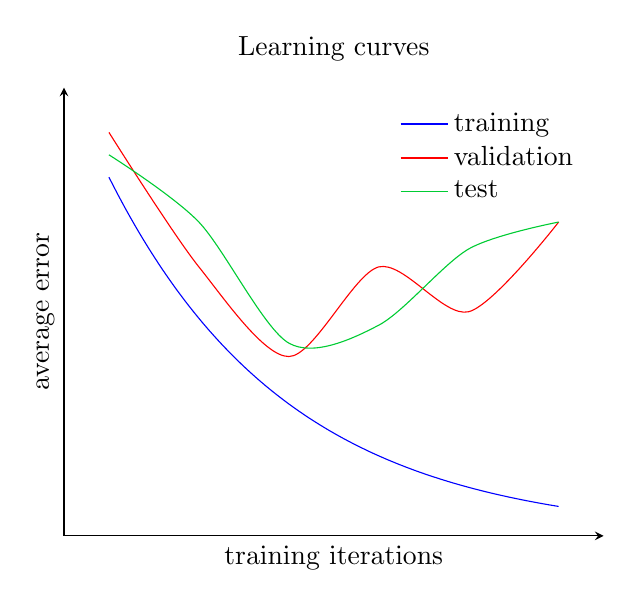
\begin{tikzpicture}[baseline]
	\begin{axis}[
			title ={Learning curves},
			xlabel={training iterations},
			ylabel={average error},
			axis x line=bottom,
			axis y line=left,
			domain=0:5,
			xmin=-0.5, xmax=5.5,
			ymin=0,	ymax=1,
			ticks=none,
			legend style={draw=none},
			legend pos= north east,
			legend entries={training,validation,test},
			legend cell align=left,
		]

		\addplot [blue, samples=101, smooth]	{.8*exp(-0.5*x)};
		
		\addplot [red, smooth] coordinates {
			(0.0,0.9)
			(1.0,0.6)
			(2.0,0.4)
			(3.0,0.6)
			(4.0,0.5)
			(5.0,0.7)
		};
		
		\addplot [green!80!blue, smooth] coordinates {
			(0.0,0.85)
			(1.0,0.7)
			(2.0,0.43)
			(3.0,0.47)
			(4.0,0.64)
			(5.0,0.7)
		};
		
	\end{axis}
\end{tikzpicture}
	\caption{The learning curves are the value of the loss function, or criterion, as a function of the training iterations.
	Both the validation and the test error are usually higher than the error on the training set.
	Sometimes, to avoid overfitting, the training procedure is stopped at a minimum of the validation learning curve \cite{duda2012pattern}.
	}
	\label{fig:LVTcurves}
\end{figure}

\subsection{Datasets}
\label{ssec:Datasets}
Creating a dataset and splitting it into subsets is another problem to deal with.
It is not so simple and straightforward as it appears.
For example a dataset which is too big will lead to a longer training time for the network, whereas a too little set will cause a poor training.

The most naive division is in three equal parts, since three are the phases of preparation for any artificial neural network.
However, as shown later in \autoref{ssec:PyDataset}, when the resources dictates otherwise, other subdivision can be implemented.
In my case, the decision was to follow the suggestions of the authors of the dataset and divide the examples into a training set and a test set only, with a ratio between the two close to 50\%.

\section{Feedforward NN}
\label{sec:Feedforward_NN}

The first and most simple type of neural network is called Feedforward.
In this kind of neural network, nodes are divided into groups called \textit{layers}.
A layer is a collection of nodes that accepts inputs from a preceding group and generate as many outputs as the number of nodes in the layer.
Each layer of a Feedforward neural network is connected in series with the others, except for the input layer at the beginning and the output layer at the end.
As for the single nodes, the inner layer are called hidden, because usually not accessible.

The information travels from the input to the output and gets elaborated from each hidden layer: there are neither connection between nodes of the same layer, nor loops or feedback between layers.
%Depending on the topology of the network, there might be more or less layers, each composed by the same or a different number of nodes.
The number of hidden layers and the number of nodes they contain depends on the network topology.
Moreover the connection between the layers might be complete, i.e. each node in the layer accepts each input of the preceding layer, in that case the layer is said to be \textit{fully connected}, or sparse as in the case of convolutional layers (see \autoref{par:Convolutional}).

\subsection{Perceptron}
\label{ssec:Perceptron}

The most naive topology of a Feedforward neural network is given by the so called \textit{Perceptron}.
The Perceptron dates back to the 1957, when the homonym \textit{Perceptron algorithm} was software implemented by Frank Rosenblatt on a computer (IBM 704) and only subsequently in hardware as the \textit{Mark 1 perceptron} \cite{frank1957perceptron,Rosenblatt1958}.
The graph of a generic (single layer) perceptron \acs{ANN} is shown in \autoref{fig:Perceptron}.

\begin{figure}[ht]
	\centering
	\tikzsetnextfilename{PerceptronNN}
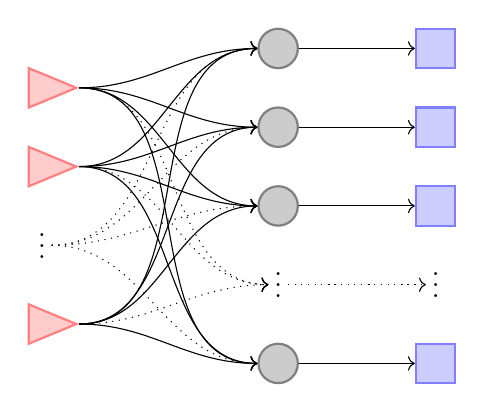
\begin{tikzpicture}
	[%
	input/.style ={isosceles triangle,	draw=red!50,		fill=red!20,		thick,	inner sep=0pt,	minimum size=5mm},%
	inner/.style ={circle,							draw=black!50,	fill=black!20,	thick,	inner sep=0pt,	minimum size=5mm},%
	output/.style={rectangle,					draw=blue!50,	fill=blue!20,	thick,	inner sep=0pt,	minimum size=5mm},%
	]

	\newcommand\lin{0}
	\newcommand{\lhid}{3}
	\newcommand{\lout}{5}
	
	% nodes
	\foreach \i in {0,1,3} \node (input\i) at (\lin,2.5-\i) [input] {};
	
	\foreach \i in {0,1,2,4} \node (inner\i) at (\lhid,3-\i) [inner] {};
	
	\foreach \i in {0,1,2,4} \node (output\i) at (\lout,3-\i) [output] {};
	
	\node (input2)		at (\lin,0.5) {}; 		\node at (\lin,0.6) {$\vdots$};
	\node (inner3)		at (\lhid,0.0) {}; 	\node at (\lhid,0.1) {$\vdots$};
	\node (output3)	at (\lout,0.0) {}; 	\node at (\lout,0.1) {$\vdots$};
	
	% interconnections
	\foreach \i in {0,1,3}%
		\foreach \j in {0,1,2,4}%
			\draw [->] (input\i) to [out=0, in=180] (inner\j);
	
	\foreach \i in {0,1,3}%
		\draw [dotted, ->] (input\i)	to [out=0, in=180] (inner3);
	\foreach \j in {0,1,2,4}%
		\draw [dotted, ->] (input2) 	to [out=0, in=180] (inner\j);
	\foreach \i in {0,1,2,4}%
		\draw [->] (inner\i) to [out=0, in=180] (output\i);
	\draw [dotted, ->] (inner3) to [out=0, in=180] (output3);
	
\end{tikzpicture}
	\caption{%
		Perceptron type neural network: in this representation the perceptron has $n$ inputs and $m$ outputs as well as a hidden layer with $m$ nodes. %
%		Colors, shape and styles are the same as in \autoref{fig:generic_NN} \vpageref{fig:generic_NN}.%
		}
	\label{fig:Perceptron}
\end{figure}

By adding more than one hidden perceptron layer to the neural network, one obtain the so called \acfi{MLP}.
This allows for more computational complexity \ref{}.
When the total number of layer is more than two, the network is called \textit{deep}.
A deep \acs{MLP} is shown in \autoref{fig:deepMLP}.
In principle any shape is possible, i.e. each layer could have a different number of nodes, however often the layers at the beginning are wider than the layer at the end of the network \ref{}.
Besides the shape, in literature a perceptron is almost always considered fully connected \ref{}.

\begin{figure}[ht]
	\centering
	\tikzsetnextfilename{MLPNN}
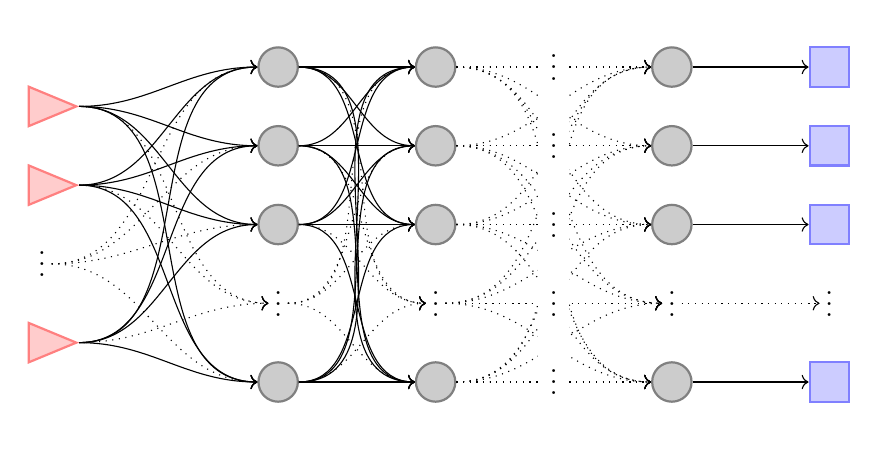
\begin{tikzpicture}
	[%
	input/.style ={isosceles triangle,	draw=red!50,		fill=red!20,		thick,	inner sep=0pt,	minimum size=5mm},%
	inner/.style ={circle,							draw=black!50,	fill=black!20,	thick,	inner sep=0pt,	minimum size=5mm},%
	output/.style={rectangle,					draw=blue!50,	fill=blue!20,	thick,	inner sep=0pt,	minimum size=5mm},%
	]

	\newcommand\lin{0}
	\newcommand{\lhid}{3}
	\newcommand{\lhidb}{5}
	\newcommand{\lhidc}{6.5}
	\newcommand{\lhidd}{8}
	\newcommand{\lout}{10}
	
	% nodes
	\foreach \i in {0,1,3} \node (input\i) at (\lin,2.5-\i) [input] {};
	
	\foreach \j in {\lhid,\lhidb,\lhidd}%
		\foreach \i in {0,1,2,4} \node (inner\j_\i) at (\j,3-\i) [inner] {};
	
	\foreach \i in {0,1,2,4} \node (output\i) at (\lout,3-\i) [output] {};
	
	\node (input2)		at (\lin,0.5) {}; 		\node at (\lin,0.6) {$\vdots$};
	\foreach \j in {\lhid,\lhidb,\lhidd}%
		\node (inner\j_3)		at (\j,0.0) {};
	\foreach \j in {\lhid,\lhidb,\lhidd}%
		\node at (\j,0.1) {$\vdots$};
	\node (output3)	at (\lout,0.0) {}; 	\node at (\lout,0.1) {$\vdots$};
	
	% interconnections
	% in - hid1
	\foreach \i in {0,1,3}%
		\foreach \j in {0,1,2,4}%
			\draw [->] (input\i) to [out=0, in=180] (inner\lhid_\j);
	\foreach \i in {0,1,3}%
		\draw [dotted, ->] (input\i)	to [out=0, in=180] (inner\lhid_3);
	\foreach \j in {0,1,2,4}%
		\draw [dotted, ->] (input2) 	to [out=0, in=180] (inner\lhid_\j);
	
	\foreach \i in {0,1,2,4}%
		\foreach \j in {0,1,2,4}%
			\draw [->] (inner\lhid_\i) to [out=0, in=180] (inner\lhidb_\j);
	\foreach \i in {0,1,2,4}%
		\draw [dotted, ->] (inner\lhid_\i)	to [out=0, in=180] (inner\lhidb_3);
	\foreach \j in {0,1,2,4}%
		\draw [dotted, ->] (inner\lhid_3) to [out=0, in=180] (inner\lhidb_\j);
	
	\foreach \i in {0,1,2,3,4}%
		\foreach \j in {0,1,2,3,4}%
			\draw [dotted,->] (inner\lhidb_\i) to [out=0, in=180] (inner\lhidd_\j);
	\fill [white] (6.3,-1.5) rectangle (6.7,3.5);
	\foreach \i in {-0.9,0.1,1.1,2.1,3.1}%
		\node at (\lhidc,\i) {$\vdots$};

	\foreach \i in {0,1,2,4}%
		\draw [->] (inner\lhidd_\i) to [out=0, in=180] (output\i);

	\draw [dotted, ->] (inner\lhidd_3) to [out=0, in=180] (output3);
	
\end{tikzpicture}
	\caption{	Deep \acf{MLP}, fully connected.}
	\label{fig:deepMLP}
\end{figure}

\subsubsection{Other Feedforward NNs}
\label{sssec:Other_Feedforward_NNs}

Feedforward neural networks are a large family that includes many other types besides the perceptron one.
A few names are autoencoder, time delay, and convolutional neural networks.
Autoencoders \acsp{ANN} are feedforward networks with the same number of input and output nodes, with the purpose of reconstructing its own inputs.
For this reason autoencoders employ unsupervised learning.
Time delay networks have a feedforward structure and their purpose is to analyze patterns in

\paragraph{Convolutional}\label{par:Convolutional} networks are inspired to the visual cortex, in which neurons are not fully connected their inputs but only to a restricted region.
Convolutional neural networks are a type of feedforward network conceived to recognize images without being misled by distortions such as translation, skewing, or scaling.
Its input is often represented as a 2D matrix, instead of a 1D vector.
This kind of network is usually composed by many layers, the prevalent kind is the convolutional one.
This layer performs a two-dimensional convolution over the input matrix of a second 2D matrix of weights, called \textit{feature map}.
Thus, each node of the layer operates on a restricted region to understand if a feature is present or not.
Commonly the operating regions are overlapping and the feature map is shared among the nodes in the same layer.

\begin{figure}[ht]
	\centering
	\tikzsetnextfilename{ConvNN}
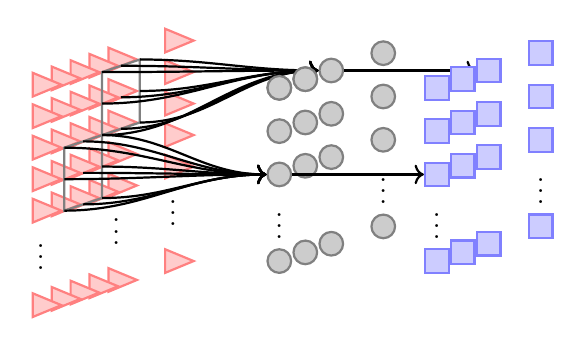
\begin{tikzpicture}[
		baseline,
		input/.style ={isosceles triangle,	draw=red!50,		fill=red!20,		thick,	inner sep=0pt,	minimum size=3mm},
		inner/.style ={circle,							draw=black!50,	fill=black!20,	thick,	inner sep=0pt,	minimum size=3mm},
		output/.style={rectangle,					draw=blue!50,	fill=blue!20,	thick,	inner sep=0pt,	minimum size=3mm},
	]

	\newcommand\lin{0}
	\newcommand{\lhid}{3}
	\newcommand{\lout}{5}
	
	%	vdots
	\foreach \x in {0,3,7}
			\node at (\lin-0.4*0.6*\x,0.4*1.8-0.4*0.2*\x) {$\vdots$};
	\foreach \z in {\lhid, \lout}
		\foreach \x in {1,5}
				\node at (\z-0.55*0.6*\x,0.55*2.0-0.55*0.2*\x) {$\vdots$};
	
	% nodes
	\foreach \x/\xt in {0/n,3,4,5,6,7}
		\foreach \y/\yt in {0/n,3,4,5,6,7}
			\node [input] (input\xt_\yt) at (\lin-0.4*0.6*\x,0.4*\y-0.4*0.2*\x) {};
	
	\foreach \x/\xt in {1/n,3,4,5}
		\foreach \y/\yt in {1/n,3,4,5}
			\node [inner] (inner\xt_\yt) at (\lhid-0.55*0.6*\x,0.55*\y-0.55*0.2*\x) {};
			
	\foreach \x/\xt in {1/n,3,4,5}
		\foreach \y/\yt in {1/n,3,4,5}
			\node [output] (output\xt_\yt) at (\lout-0.55*0.6*\x,0.55*\y-0.55*0.2*\x) {};
	
	% interconnections

	\draw [black!50,thick] (input3_5.east) -- (input5_5.east)%
		-- (input5_7.east) -- (input3_7.east) -- cycle;
%	\draw [black!50,thick] (input4_4.east) -- (input4_6.east)%
%		-- (input6_6.east) -- (input6_4.east) -- cycle;
	\draw [black!50,thick] (input5_3.east) -- (input5_5.east)%
		-- (input7_5.east) -- (input7_3.east) -- cycle;	
	
	\foreach \xt in {3,4,5}
		\foreach \yt in {5,6,7}
			\draw [thick,->] (input\xt_\yt)	to [out=0, in=180] (inner3_5);	
	
%	\foreach \xt in {4,5,6}
%		\foreach \yt in {4,5,6}
%			\draw [thick,->] (input\xt_\yt)	to [out=0, in=180] (inner4_4);

	\foreach \xt in {5,6,7}
		\foreach \yt in {3,4,5}
			\draw [thick,->] (input\xt_\yt)	to [out=0, in=180] (inner5_3);
		
	%orange!80!red
	%green!90!blue
	\draw [thick,->] (inner5_3) to [out=0, in=180] (output5_3);
	\draw [thick,->] (inner3_5) to [out=0, in=180] (output3_5);
		
	% redraw some things
	
	\node [inner] at (inner5_5) {};
	\node [inner] at (inner4_5) {};
	\node [output] at (output5_5) {};
	\node [output] at (output4_5) {};
	
\end{tikzpicture}
	\caption{%
		Pictorial representation of a layer of a convolutional supernode.
		Several supernodes might be placed side by side to form a convolutional layer.
		}
	\label{fig:convolutionalNN}
\end{figure}

Convolutional neural networks are nowadays widely used in image recognition with outstanding results and they improve with a steady pace.
A technological application of this kind of network is the real time recognition of obstacles in a vehicle path, for safety and automation purposes in the automotive industry.

\subsection{Other Types of NNs}
\label{ssec:Other_Types_of_NNs}
By changing the topology of the nodes distribution and their connections, one obtain other networks that cannot be catalogued under the class of feedforward networks.
Moreover, those different types of network are not a niche, but they are widely \ref{} studied as a different approaches to the same or additional problems.

\subsubsection{Recurrent NN}
\label{sssec:Recurrent_NN}
\acp{RNN} are a kind of network in which a portion of the input of nodes depends on the (past) output of the same nodes or nodes of subsequent layers.
That is information does not propagates only forward like in the feedforward networks, but can propagate also backward, for example in loops or in feedbacks.

\begin{figure}[ht]
	\centering
	\tikzsetnextfilename{RecurrentNN}
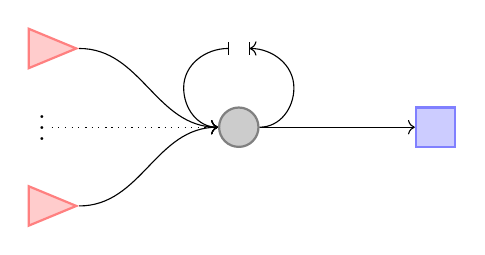
\begin{tikzpicture}
	[%
	input/.style ={isosceles triangle,	draw=red!50,		fill=red!20,		thick,	inner sep=0pt,	minimum size=5mm},%
	inner/.style ={circle,							draw=black!50,	fill=black!20,	thick,	inner sep=0pt,	minimum size=5mm},%
	output/.style={rectangle,					draw=blue!50,	fill=blue!20,	thick,	inner sep=0pt,	minimum size=5mm},%
	]

	\newcommand\lin{0}
	\newcommand{\lhid}{2.5}
	\newcommand{\lout}{5}
	
	% nodes
	\foreach \i in {0,2} \node (input\i) at (\lin,1-\i) [input] {};
	\node (input1)		at (\lin, 0) {}; 		\node at (\lin, 0.1) {$\vdots$};
	
	\node (inner1) at (\lhid, 0) [inner] {};
	
	\node (output1) at (\lout, 0) [output] {};
	
	% interconnections
	\foreach \i in {0,2}%
		\draw [->] (input\i) to [out=0, in=180] (inner1);
	\draw [dotted, ->] (input1)	to [out=0, in=180] (inner1);
	
	\node (delay) at (\lhid, 1) {};
	\draw [->|] (inner1) to [out=  0, in=270] +(0.7,0.5)   to [out= 90, in=  0] (delay);
	\draw [|->] (delay)  to [out=180, in= 90] +(-0.7,-0.5) to [out=270, in=180] (inner1);
	
	\draw [->] (inner1) to [out=0, in=180] (output1);
	
\end{tikzpicture}
	\caption{%
		Representation of a recurrent node.
		One of the inputs is given by the output itself.
		This output to input connection could be mediated by a delay device, so that for example the output at $t-1$ becomes the input at $t$.
		Depending on the structure of the network, there might be recurrent nodes and/or recurrent groups of nodes, i.e. loops.
		}
	\label{fig:RecurrentNN}
\end{figure}

Recurrent networks have found greatest use in time series analysis and prediction \cite{duda2012pattern}.
However often recurrent type of networks are employed to obtain the same classification of feedforward ones.
In this case, the former are equivalent to the latter, if ``unfolded'' in time.
That is the expansion of the recurrent architecture in time is the same as the topology of the feedforward one in space.

\subsubsection{Reservoir NN}
\label{sssec:Reservoir_NN}
Reservoir neural networks, or \ac{RC}, differ from feedforward and recurrent networks in the learning approach.
In fact, the topology of a reservoir network could be exactly the same as that of a deep multi-layer perceptron or that of a recurrent network.
However, the reservoir computing differs in approach in respect to deep learning.
It claims that it is not necessary to learn all the weights of the network, as in deep learning, but it is sufficient to train only the last (perceptron) layer of the network.

\begin{figure}[ht]
	\centering
	\tikzsetnextfilename{ReservoirNN}
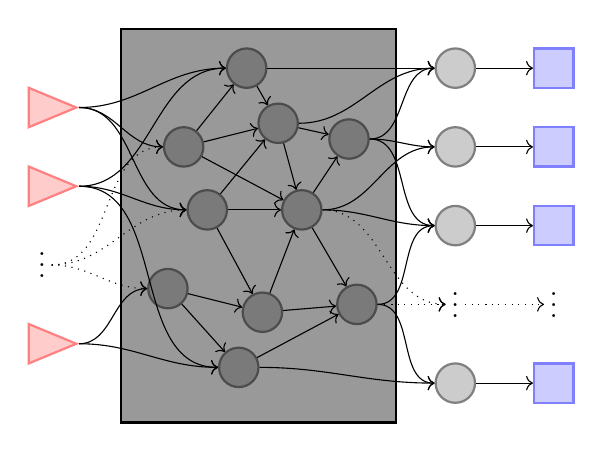
\begin{tikzpicture}
	[%
	input/.style ={isosceles triangle,	draw=red!50,		fill=red!20,		thick,	inner sep=0pt,	minimum size=5mm},%
	inner/.style ={circle,							draw=black!50,	fill=black!20,	thick,	inner sep=0pt,	minimum size=5mm},%
	output/.style={rectangle,					draw=blue!50,	fill=blue!20,	thick,	inner sep=0pt,	minimum size=5mm},%
	]

	\newcommand\lin{0}
	\newcommand\lhid{5.25}
	\newcommand{\lout}{6.5}
	
	% nodes
	\foreach \i in {0,2,3} \node (input\i) at (\lin,0.5+\i) [input] {};
	
	\foreach \i in {0,2,3,4} \node (output\i) at (\lout,\i) [output] {};
	
	\foreach \n/\x/\y in {	0/1.6/1.2, 1/1.8/3.0, 2/2.1/2.2, 3/2.5/0.2, 4/2.6/4.0, %
												5/2.8/0.9, 6/3.0/3.3, 7/3.3/2.2, 8/3.9/3.1, 9/4.0/1.0, %
												10/\lhid/0, 12/\lhid/2, 13/\lhid/3, 14/\lhid/4 %
												}
			\node (inner\n) at (\x,\y) [inner] {};
	
	\node (input1)		at (\lin,1.5) {}; 		\node at (\lin,1.6) {$\vdots$};
	\node (inner11)	at (\lhid,1.0) {}; 	\node at (\lhid,1.1) {$\vdots$};
	\node (output1)	at (\lout,1.0) {}; 	\node at (\lout,1.1) {$\vdots$};
	
	% interconnections
	% input to inner
	\foreach \i/\o in {0/0, 0/3, 2/2, 2/3, 2/4, 3/1, 3/2, 3/4}
		\draw [->] (input\i) to [out=0,in=180] (inner\o);
		
	\foreach \i/\o in {1/0, 1/1, 1/2}
		\draw [dotted, ->] (input\i) to [out=0,in=180] (inner\o);

	% inner to inner
	\foreach \i/\o in {	0/3, 0/5, 1/4, 1/6, 1/7, 2/5, 2/6, 2/7,%
											3/9, 4/6, 5/7, 5/9, 6/7, 6/8, 7/8, 7/9%
											}
		\draw [->] (inner\i) to (inner\o);
		
	\foreach \i/\o in {3/10, 9/10, 7/12, 8/12, 9/12, 7/13, 8/13, 4/14, 6/14, 8/14}
		\draw [->] (inner\i) to [out=0,in=180] (inner\o);
				
	\foreach \i/\o in {7/11, 9/11}
		\draw [dotted, ->] (inner\i) to [out=0,in=180] (inner\o);

	% inner to output
	\foreach \ii in {0, 2, 3, 4}
		\draw [->] (inner1\ii) to [out=0,in=180] (output\ii);
	\draw [dotted, ->] (inner11)  to [out=0,in=180] (output1);
	
	% black box
	\filldraw [thick, draw=black, fill=black, fill opacity=0.4] (1.0,-0.5) rectangle (4.5,4.5);
	
\end{tikzpicture}
	\caption{A reservoir NN is topologically equivalent to deep networks. However only the last layer is trained. In this picture the trained node are represented outside the box, while those inside are initialized with random weights which are then left unchanged.}
	\label{fig:reservoirNN}
\end{figure}

\noindent This kind of networks, then, can be trained much faster than their respective counterparts, i.e. feedforward and recurrent.
The question over which training method is correct is still debated and literature does not provide clear answers yet.

%\subsubsection{Modular NN}
%\label{sec:Modular_NN}

%\subsubsection{Spiking NN}
%\label{sec:Spiking_NN}
%Spiking artificial networks are the most different kind in respect to all the other networks until now described.
%In this class of ANNs, information is not coded only in the intensity of the signal, but also in the rate of signals, e.g. a high value will be encoded as a signal with high repetition rate, whereas a low value as a signal with low repetition rate.
%This way of encoding information is more alike the mechanism of biological neural networks, such as our brain \ref{}.
%
%\vspace{1em}
%\noindent LOOK INTO other type of neuron model: Hodgkin–Huxley (H-H) model\\
%\url{ https://en.wikipedia.org/wiki/Binding_neuron }

%\section{Real-Life Examples}
%\label{sec:Real-Life_Examples}
%\noindent\uppercase{\large{? Should I keep this section ?}}
%\normalsize

\section{ANN Simulation}
\label{sec:ANN_Simulation}
In the field of artificial neural network simulation, there are several platforms that are independently developed.
Among them there are TensorFlow, Theano, Caffe, Keras, Torch, and PyTorch.
Unfortunately, each one of them have its strength and weakness, therefore the choice of the framework becomes very difficult.

To make a choice, the key factors considered were the language used, the features, the flexibility, and the level of diffusion of the framework in the machine learning community.
The language used is a determining factor, because it takes time to learn the peculiarities of a library written for a known language, but even more time to learn to use an unknown programming language.
However also the features and the flexibility in the implementation are important traits, on account of the fact that any feature that is not natively implemented needs new coding.
In turn, it is difficult to integrate new coding if the framework is not flexible enough to accommodate extensions or custom definitions.
Last, but not least, it is easier to find support for a widespread framework in respect to a limitedly used one.
In regards to this, \autoref{fig:GoogleTrendsPyTorch} shows the number of internet searches for some frameworks in the past few years.

In light of the facts above, PyTorch was chosen as framework.
PyTorch is an open source machine learning library for python, which development has started only recently and it is based upon the older framework Torch  \cite{PyTorch.org}.
It provides a high-level platform for the deep learning ecosystem and integrates acceleration libraries that allow fast and lean operation, both on common \acsp{CPU} and \acsp{GPU}.
It is based on a backpropagation algorithm called \textit{Reverse-mode auto-differentiation}, which allows versatile execution.

To summarize, the library was chosen for its language, its flexibility, and the growing interest for it within the machine learning community.
Nevertheless, its features make it a very powerful framework. However, considering the need to keep the simulated system as simple as possible, this last characteristic slipped in the background.
The need to simulate a simple network comes from the fact that the ultimate goal of this project is to implement an \acs{ANN} with a (photonic) hardware architecture.

\begin{figure}[htbp]
	\centering
	\tikzsetexternalprefix{tikz/}	% set subfolder
\tikzsetnextfilename{GoogleTrendsPyTorch}

\begin{tikzpicture}[baseline]
	
	\begin{axis}[
			title={Google Trends Analytics},
			xlabel={Year},
			ylabel={Interest over time},
%			tick align=outside,
			width=\textwidth*0.75,%
			height=207pt,
			legend style={at={(0.5,-0.45)},anchor=north,legend columns=-1},
			date coordinates in=x,
			xtick distance={124},
			xticklabel={\month-\year},
			xticklabel style= {rotate=90,anchor=near xticklabel},
		]
			 
		\addplot [semithick, blue!80]
			table [x index=0, y index=1] {tikz/GTrends_multiTimeline.csv};
		\addplot [semithick, red]
			table [x index=0, y index=2] {tikz/GTrends_multiTimeline.csv};
		\addplot [semithick, orange]
			table [x index=0, y index=3] {tikz/GTrends_multiTimeline.csv};
		\addplot [semithick, green!60!blue]
			table [x index=0, y index=4] {tikz/GTrends_multiTimeline.csv};
		\addplot [semithick, black]
			table [x index=0, y index=5] {tikz/GTrends_multiTimeline.csv};
			
    \addlegendentry{ \scriptsize PyTorch }
    \addlegendentry{ \scriptsize TensorFlow }
    \addlegendentry{ \scriptsize Theano }
    \addlegendentry{ \scriptsize Keras }
    \addlegendentry{ \scriptsize Caffe }
    
	\end{axis}
\end{tikzpicture}
	\caption{Google Search statistics for different keywords in the \textit{machine learning and artificial intelligence} field.
		Numbers represent search interest relative to the highest point on the chart for the given region and time.
		A value of 100 is the peak popularity for the term.}
	\label{fig:GoogleTrendsPyTorch}
\end{figure}

%The resources and the time available allowed me to implement physically only the activation function of one node.
%Hence, to test this hardware implementation as I will show in \autoref{sec:Test_of_a_Trained ANN} of \autoref{ch:experiments}, I had first to simulate and train \textit{offline} a specific neural network.
%To do so, I chose a programming language, \textit{Python}, and a library, \textit{PyTorch}, which helped me in this task.

\subsection{PyTorch}
\label{ssec:PyTorch}
PyTorch is a Python package which provides a powerful framework for deep learning.
It is versatile in the sense that allow customizations at almost every level of operation.
For the purposes of this work, a neural network implemented in PyTorch is composed by the definition of three main components and a few lines of code to implement the operation.

The most important part of the network is the so called \textit{model}, which defines the topology of the network by setting parameters such as the number of nodes in each layer and the connections among them.
Moreover, it defines also the activation function for each node, separately or in groups.
The activation function can be coded from scratch, but can also be one of the functions provided by the library or a composition of them.
While the first offers almost unlimited flexibility, the second choice consents to exploit the functions already given.
The second option is the best choice, if the needs of the task support it, because it allows to save much time.

Another important part of the network is the so called \textit{criterion}, which is nothing else than the loss function.
The set of functions provided by PyTorch can accommodate almost any necessity.
Moreover, their operation can usually be adjusted with some internal parameters.

Similarly to the criterion, the last piece of the system is given by the \textit{optimizer}.
Optimizers are a class of algorithms that provides the optimization of the weights during the learning phase.
Most commonly used methods are already supported and they provide parameters to fine tune their execution.

Following the official tutorials and the immense package documentation, I implemented a fully connected \acf{MLP} model and then tested it with randomly generated numbers until its operation seemed correct.
The code that I implemented allows to change the overall structure of the network with some parameters (see \autoref{ssec:Simulated_ANN_operation})
The optimizer chosen is called \acfi{SGD}, which is parametrized just by the learning rate, at least in its vanilla implementation.
The criterion used initially was the mean square error, however it was eventually replaced by the \acfi{CEL}, which is more suited to the classification task.

\subsection{Dataset}
\label{ssec:PyDataset}
Initial tests and trials on artificial neural networks are often made by using randomly generated sets of numbers.
However, once the system has been successfully set up, to compare different working parameters such as number of nodes and number of layers, a common standardized dataset should be employed.
Moreover in this way, it is possible to compare implementations belonging to other research groups.

Again, the need to keep the system as simple as possible, drove my attention towards datasets of middle to small sizes.
With the help of the \textit{UC Irvine Machine Learning Repository} \cite{UCIMLR}, I selected one with a bit less than a thousand entries.
The dataset is called \textit{Connectionist Bench (Vowel Recognition - Deterding Data) Data Set}.
It is composed by \num{990} entries of \num{10} attributes, i.e. input values, grouped in \num{11} classes.

Each entry is a vector of \num{10} real numbers plus an integer number between \num{0} and \num{10}.
In view of the fact the proposed activation function is a real-positive-valued function (see \autoref{sec:Characterization_of_the_Activation_Function}), I renormalized the database.
The normalization is independently applied to each one of the attributes in such a way that is described by a real number in $[0,1]$.
The normalization is applied before the dataset is divided in the learning and testing examples.

The authors suggest to divide the dataset a learning set of \num{528} entries and a testing set of \num{462} entries.
Since the number of entries is low, compared to other datasets, the validation set is not define.
In this case, the test set is used as validation instead too.

\subsection{Simulated ANN operation}
\label{ssec:Simulated_ANN_operation}
The model that I defined allows some changes with the simple definition of a few parameters.
Specifically, the parameters cover the number of input and ouptut nodes, the number of hidden layer, and the number of nodes in each hidden layer.
Whereas the number of input and output nodes is defined by the problem, i.e. the dataset, the other are free parameters that can
Another degree of freedom that I implemented is whether the last hidden layer applies the nonlinear activation function or just the weighted sum, since I observed that many network in the tutorials were built this way.
The scheme of the network is shown in \autoref{fig:ANN_model}.

\begin{figure}[htbp]
	\centering
	\tikzsetnextfilename{PT_MLP}%	
%	% nodes
%	\foreach \i in {0,1,3} \node (input\i) at (\lin,2.5-\i) [input] {};
	
%	\foreach \j in {\lhid,\lhidb,\lhidd}
%		\foreach \i in {0,1,2,4} \node (inner\j_\i) at (\j,3-\i) [inner] {};
%	\foreach \j in {\lhide}%
%	\foreach \i in {0,1,3} \node (inner\lhide_\i) at (\lhide,2.5-\i) [inner] {};
%	
%	\foreach \i in {0,1,3} \node (output\i) at (\lout,2.5-\i) [output] {};
%	
%	\node (input2)		at (\lin,0.5) {}; 		\node at (\lin,0.6) {$\vdots$};
%	\foreach \j in {\lhid,\lhidb,\lhidd}%
%		\node (inner\j_3)		at (\j,0.0) {};
%	\foreach \j in {\lhid,\lhidb,\lhidd}%
%		\node at (\j,0.1) {$\vdots$};
%	\node (inner\lhide_2) at (\lhide,0.5){}; \node at (\lhide,0.6) {$\vdots$};
%	\node (output2)	at (\lout,0.5) {}; 	\node at (\lout,0.6) {$\vdots$};
	
	% interconnections
	% in - hid1
%	\foreach \i in {0,1,3}%
%		\foreach \j in {0,1,2,4}%
%			\draw [->] (input\i) to [out=0, in=180] (inner\lhid_\j);
%	\foreach \i in {0,1,3}%
%		\draw [dotted, ->] (input\i)	to [out=0, in=180] (inner\lhid_3);
%	\foreach \j in {0,1,2,4}%
%		\draw [dotted, ->] (input2) 	to [out=0, in=180] (inner\lhid_\j);
%	
%	\foreach \i in {0,1,2,4}%
%		\foreach \j in {0,1,2,4}%
%			\draw [->] (inner\lhid_\i) to [out=0, in=180] (inner\lhidb_\j);
%	\foreach \i in {0,1,2,4}%
%		\draw [dotted, ->] (inner\lhid_\i)	to [out=0, in=180] (inner\lhidb_3);
%	\foreach \j in {0,1,2,4}%
%		\draw [dotted, ->] (inner\lhid_3) to [out=0, in=180] (inner\lhidb_\j);
%	
%	\foreach \i in {0,1,2,3,4}%
%		\foreach \j in {0,1,2,3,4}%
%			\draw [dotted,->] (inner\lhidb_\i) to [out=0, in=180] (inner\lhidd_\j);
%	\fill [white] (6.3,-1.5) rectangle (6.7,3.5);
%	\foreach \i in {-0.9,0.1,1.1,2.1,3.1}%
%		\node at (\lhidc,\i) {$\vdots$};
%
%%	\foreach \i in {0,1,3}%
%%		\draw [->] (inner\lhidd_\i) to [out=0, in=180] (output\i);
%	\foreach \i in {0,1,3}%
%		\draw [->] (inner\lhide_\i) to [out=0, in=180] (output\i);
%
%	\draw [dotted, ->] (inner\lhide_2) to [out=0, in=180] (output2);
	
%\end{tikzpicture}

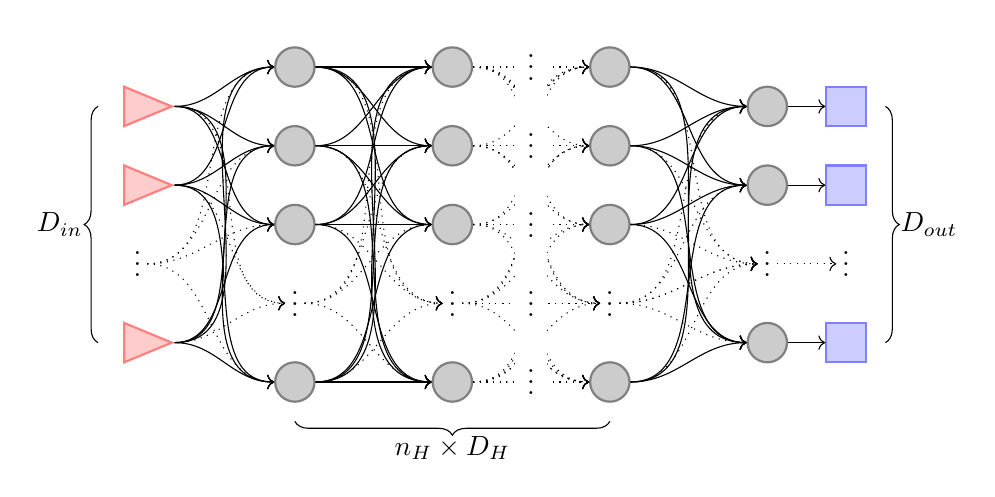
\begin{tikzpicture}
	[%
	input/.style ={isosceles triangle,	draw=red!50,		fill=red!20,		thick,	inner sep=0pt,	minimum size=5mm},%
	inner/.style ={circle,							draw=black!50,	fill=black!20,	thick,	inner sep=0pt,	minimum size=5mm},%
	output/.style={rectangle,					draw=blue!50,	fill=blue!20,	thick,	inner sep=0pt,	minimum size=5mm},%
	]

	\newcommand{\lin}{0}
	\newcommand{\lhid}{2}
	\newcommand{\lhidb}{4}
	\newcommand{\lhidc}{5}
	\newcommand{\lhidd}{6}
	\newcommand{\lhide}{8}
	\newcommand{\lout}{9}
	
	% nodes
	\foreach \i in {0,1,3} \node (input\i) at (\lin,2.5-\i) [input] {};
	
	\foreach \j in {\lhid,\lhidb,\lhidd}%
		\foreach \i in {0,1,2,4} \node (inner\j_\i) at (\j,3-\i) [inner] {};
	\foreach \i in {0,1,3} \node (inner\lhide_\i) at (\lhide,2.5-\i) [inner] {};
	\foreach \i in {0,1,3} \node (output\i) at (\lout,2.5-\i) [output] {};
	
	\node (input2)		at (\lin,0.5) {}; 		\node at (\lin,0.6) {$\vdots$};
	\foreach \j in {\lhid,\lhidb,\lhidd}%
		\node (inner\j_3)		at (\j,0.0) {};
	\foreach \j in {\lhid,\lhidb,\lhidd}%
		\node at (\j,0.1) {$\vdots$};
	\node (inner\lhide_2) at (\lhide,0.5){}; \node at (\lhide,0.6) {$\vdots$};
	\node (output2)	at (\lout,0.5) {}; 	\node at (\lout,0.6) {$\vdots$};
	
	% interconnections
	% in - hid1
	\foreach \i in {0,1,3}%
		\foreach \j in {0,1,2,4}%
			\draw [->] (input\i) to [out=0, in=180] (inner\lhid_\j);
	\foreach \i in {0,1,3}%
		\draw [dotted, ->] (input\i)	to [out=0, in=180] (inner\lhid_3);
	\foreach \j in {0,1,2,4}%
		\draw [dotted, ->] (input2) 	to [out=0, in=180] (inner\lhid_\j);
	
	\foreach \i in {0,1,2,4}%
		\foreach \j in {0,1,2,4}%
			\draw [->] (inner\lhid_\i) to [out=0, in=180] (inner\lhidb_\j);
	\foreach \i in {0,1,2,4}%
		\draw [dotted, ->] (inner\lhid_\i)	to [out=0, in=180] (inner\lhidb_3);
	\foreach \j in {0,1,2,4}%
		\draw [dotted, ->] (inner\lhid_3) to [out=0, in=180] (inner\lhidb_\j);
	
	\foreach \i in {0,1,2,3,4}%
		\foreach \j in {0,1,2,3,4}%
			\draw [dotted,->] (inner\lhidb_\i) to [out=0, in=180] (inner\lhidd_\j);
	\fill [white] (4.8,-1.5) rectangle (5.2,3.5);
	\foreach \i in {-0.9,0.1,1.1,2.1,3.1}%
		\node at (\lhidc,\i) {$\vdots$};
	\foreach \i in {0,1,2,3,4}%
		\draw [dotted, ->] (inner\lhidd_\i)	to [out=0, in=180] (inner\lhide_2);
	\foreach \j in {0,1,2,3}%
		\draw [dotted, ->] (inner\lhidd_3) to [out=0, in=180] (inner\lhide_\j);

	\foreach \i in {0,1,2,4}%
		\foreach \j in {0,1,3}
			\draw [->] (inner\lhidd_\i) to [out=0, in=180] (inner\lhide_\j);
	\foreach \i in {0,1,3}
			\draw [->] (inner\lhide_\i) to [out=0, in=180] (output\i);

	\draw [dotted, ->] (inner\lhide_2) to [out=0, in=180] (output2);
	
	\draw [decorate, decoration={brace, amplitude=5}] (\lhidd,-1.5) -- (\lhid,-1.5)
		node [midway, below=2pt] {$n_{H}\times D_H$};
	\draw [decorate, decoration={brace, amplitude=5}] (-.5,-0.5) -- (-.5,2.5)
		node [midway, left=2pt]  {$D_{in}$};
	\draw [decorate, decoration={brace, amplitude=5}] (9.5,2.5) -- (9.5,-0.5)
		node [midway, right=2pt] {$D_{out}$};
	
\end{tikzpicture}
	\caption{Topology of the model implemented in PyTorch. The number of input ($D_{in}$) ad output nodes ($D_{out}$), as well as the number of nodes in the last hidden layer is determined by the dataset.
	The number of nodes ($D_{H}$) in the other hidden layers and the number of hidden layers itself ($n_{H}$) is governed by a parameter.}
	\label{fig:ANN_model}
\end{figure}

The choice of the structure of the neural network is purely heuristic, since up to now no satisfactory method has been proposed in literature.
However, given the problem (dataset), at least the input and output layer have a fixed amount of nodes.
Specifically, the input nodes are \num{10}, the number of attributes, while the output nodes are \num{11}, the number of classes.

Using the chosen dataset, I tested the neural network operation on the model defined before, with two different kinds of activation function.
Initially I implemented a \acfi{ReLU} and a \textit{Logistic} (sigmoid) activation functions.
The \acs{ReLU} function is a standard activation function and is defined as follows:
\begin{equation}
f_{ReLU}(x) =
\begin{cases}
	0 & \qquad \mathrm{for}~ x\leq 0\\
	x & \qquad \mathrm{for}~ x\geq 0
\end{cases}~.
\label{eq:relu}
\end{equation}
On the other hand, the Logistic function, which has already been shown in \autoref{fig:activation_function_example_2}, is defined by
\begin{equation}
f_{Logistic}(x) = \frac{1}{1+e^{-k\left(x-x_0\right)}},
\end{equation}
with the parameters $k\in \mathcal{R}^+$ and $x_0\in \mathcal{R}$.
Both functions are widely used in literature, however the \acs{ReLU} function seems to be preferred lately.
I will discuss in \autoref{sec:Test_of_a_Trained ANN} the results of the same network models, with the nonlinear activation function given by the microring resonator.

\subsubsection{Learning}
After the definition of the model, I had to train the networks on the training set.
Since the dataset is small, all the examples are fed into the model, then the overall loss is evaluated, and finally the weights are upgraded.
This method is called \textit{batch} operation; others are \textit{online} operation, which evaluate the loss and change the weights at each example, and \textit{minibatch} operation, which uses a random subset of the full dataset.

Every time the network is trained on the full dataset, an \textit{epoch} is completed.
I trained the models defined above for \num{2000} epochs, in order to observe both the fast and slow dynamics.
For example, smaller networks tend to train faster, because there are less free parameters.
On the other hand, larger networks often train slower, but can obtain better results thanks to their complexity.

Moreover, I defined a different learning rates $l_r$ for each activation function, in order to provide the best parameter for different models but still be able to compare the performance of similar ones.
Specifically the learning rate for the \acs{ReLU} is $l_{r|ReLU} = \num{5e-2}$, while for the Logistic function is $l_{r|Logistic}= \num{5e-3}$

\begin{figure}[htbp]
	\centering
	\tikzsetexternalprefix{tikz/}	% set subfolder
\tikzsetnextfilename{Train_evolution}

%\newcommand{\righttriangles}[1]{
%    \pgfplotstableread[col sep=tab, header=true]{#1}{\table}
%    \pgfplotstablegetcolsof{#1}
%    \pgfmathtruncatemacro\numberofcols{\pgfplotsretval - 1}
%    \pgfplotsinvokeforeach{1,...,\numberofcols}{
%        \pgfplotstablegetcolumnnamebyindex{##1}\of{\table}\to{\colname}
%        \addplot [name path=down##1, semithick, color##1, mark=*, mark size=1, mark options={solid}]%
%        		table [x index= 0, y index=##1] {#1};
%        \addlegendentryexpanded{ \SI{\colname}{\mW} }
%    }
%}

%\newcommand{\lefttriangles}[1]{
%    \pgfplotstableread[col sep=tab, header=true]{#1}{\table}
%    \pgfplotstablegetcolsof{#1}
%    \pgfmathtruncatemacro\numberofcols{\pgfplotsretval - 1}
%    \pgfplotsinvokeforeach{1,...,\numberofcols}{
%        \pgfplotstablegetcolumnnamebyindex{##1}\of{\table}\to{\colname}
%        \addplot [name path=up##1, semithick, color##1, mark=*, mark size=1, mark options={solid}]%
%        		table [x index= 0, y index=##1] {#1};
%    }
%}

\begin{tikzpicture}[baseline]

%	\definecolor{color1}{rgb}{0.12156862745098,0.466666666666667,0.705882352941177}
%	\definecolor{color2}{rgb}{1,0.498039215686275,0.0549019607843137}
%	\definecolor{color3}{rgb}{0.172549019607843,0.627450980392157,0.172549019607843}
%	\definecolor{color4}{rgb}{0.83921568627451,0.152941176470588,0.156862745098039}
%	\definecolor{color5}{rgb}{0.580392156862745,0.403921568627451,0.741176470588235}
%	\definecolor{color6}{rgb}{0.549019607843137,0.337254901960784,0.294117647058824}
%	\definecolor{color7}{rgb}{0.890196078431372,0.466666666666667,0.76078431372549}
%	\definecolor{color8}{rgb}{0.45,0.45,0.45}
%	\definecolor{color9}{rgb}{0.25,0.25,0.99}
	
	\begin{axis}[
			title={Loss Criterion Evolution},
			xlabel={Epochs},
			ylabel={Loss},
%			tick align=outside,
%			tick pos=left,
			width=\textwidth*0.75,
			height=207pt,
			legend pos = outer north east,
%			cycle list name=color list,
			/pgf/number format/1000 sep=,
%			xmin=-199, xmax=2199,
			xtick distance=500,
			minor tick num=2,
			domain=0:4000,
			train/.style={
				smooth,
				semithick,
			},
			valid/.style={
				only marks,
				mark=o,
				mark options={scale=0.25},
				forget plot,
			},
		]
		\addlegendentry{\hspace{-.6cm}$f_{ReLU}$};
		\addlegendimage{empty legend};

%		\addplot [red, train] {0.2+2.5*exp(-0.01*x)+0.05*rand};
		\addplot [red, train] table [x index=0, y index=3] {tikz/base-11x2_learn.csv};
		\addlegendentry{$2\times 11$}
%		\addplot [red, valid] {0.4+2.3*exp(-0.01*x)+0.1*rand};
		\addplot [red, valid] table [x index=0, y index=3] {tikz/base-11x2_valid.csv};

%		\addplot [teal, train] {0.2+2.5*exp(-0.01*x)+0.05*rand};
		\addplot [teal, train] table [x index=0, y index=6] {tikz/base-11x3_learn.csv};
		\addlegendentry{$3\times 11$}
%		\addplot [teal, valid] {0.4+2.3*exp(-0.01*x)+0.1*rand};
		\addplot [teal, valid] table [x index=0, y index=6] {tikz/base-11x3_valid.csv};
		
%		\addplot [blue, train] {0.15+2.6*exp(-0.011*x)+0.06*rand};
		\addplot [blue, train] table [x index=0, y index=9] {tikz/base-22x2_learn.csv};
		\addlegendentry{$2\times 22$}
%		\addplot [blue, valid] {0.35+2.35*exp(-0.012*x)+0.13*rand};
		\addplot [blue, valid] table [x index=0, y index=9] {tikz/base-22x2_valid.csv};
		
%		\addplot [cyan, train] {0.15+2.6*exp(-0.011*x)+0.06*rand};
		\addplot [cyan, train] table [x index=0, y index=7] {tikz/base-22x3_learn.csv};
		\addlegendentry{$3\times 22$}
%		\addplot [cyan, valid] {0.35+2.35*exp(-0.012*x)+0.13*rand};
		\addplot [cyan, valid] table [x index=0, y index=7] {tikz/base-22x3_valid.csv};
%		red,blue,black,yellow,brown,teal,orange,violet,cyan,green!70!black,magenta,gray
		
%		\addlegendentry{\hspace{-.6cm}$f_{Logistic}$}
%		\addlegendimage{empty legend};
%		
%		\addplot [orange, train] {1.2+1.5*exp(-0.01*x)+0.05*rand};
%		\addlegendentry{$2\times 11$}
%		\addplot [orange, valid] {1.4+1.3*exp(-0.01*x)+0.1*rand};
%		
%		\addplot [blue!20!green, train] {1.15+1.6*exp(-0.011*x)+0.06*rand};
%		\addlegendentry{$2\times 22$}
%		\addplot [blue!20!green, valid] {1.35+1.35*exp(-0.012*x)+0.13*rand};	
%		
%		\addplot [gray, train] {1.2+1.5*exp(-0.01*x)+0.05*rand};
%		\addlegendentry{$3\times 11$}
%		\addplot [gray, valid] {1.4+1.3*exp(-0.01*x)+0.1*rand};
%		
%		\addplot [violet, train] {1.15+1.6*exp(-0.011*x)+0.06*rand};
%		\addlegendentry{$3\times 22$}
%		\addplot [violet, valid] {1.35+1.35*exp(-0.012*x)+0.13*rand};
		
	\end{axis}
\end{tikzpicture}
	\caption{Evolution of the loss criterion (solid lines) throughout the epochs.
		Points represent the values of the loss criterion on the validation dataset, carried out repeatedly during the training.
	}
	\label{fig:PyTorch_learning}
\end{figure}

\autoref{fig:PyTorch_learning} shows the evolution of the loss and the validation of each model during the \num{2000} epochs of training.
From the evolution of the loss function we can see that every model has 


\subsubsection{Collection of results}
Since the number of classes is \num{11}, the percentage of correct answer given a random value is $\sim \SI{9.09}{\percent}$.
Hence, values of correct answers above that mean that the neural network is working.
On the other hand, values around or even below \SI{9.09}{\percent} mean that the current neural network is not working at all.

\autoref{tab:PyResults} collects all the results for the different topologies.
The same shape has been tested with both $f_{ReLU}$ and $f_{Logistic}$ to compare the performance.

\begin{table}[htbp]
	\centering
	\begin{tabular}{c c c c r}
	\toprule
	activation	& no. hidden 	& no. nodes	& other			& Percent\\
	function		& layers 			& per layer	& parameters	& correct\\
	\midrule
	$f_{ReLU}$ 			& 2 & 11 & - & \SI{70}{\percent}\\
	$f_{ReLU}$ 			& 2 & 22 & - & \SI{70}{\percent}\\
	$f_{ReLU}$ 			& 3 & 11 & - & \SI{70}{\percent}\\
	$f_{ReLU}$ 			& 3 & 22 & - & \SI{70}{\percent}\\
	$f_{Logistic}$ 	& 2 & 11 & - & \SI{9}{\percent}\\
	$f_{Logistic}$ 	& 2 & 22 & - & \SI{9}{\percent}\\
	$f_{Logistic}$ 	& 3 & 11 & - & \SI{9}{\percent}\\
	$f_{Logistic}$ 	& 3 & 22 & - & \SI{9}{\percent}\\
	\bottomrule
	\end{tabular}
	\caption{Results of the different activation functions and the several network topologies.
	}
	\label{tab:PyResults}
\end{table}

%+-------------------------+--------+---------+---------+
%|                         | no. of | no.     | percent |
%|       Classifier        | hidden | correct | correct |
%|                         | units  |         |         | 
%+-------------------------+--------+---------+---------+
%| Single-layer perceptron |  -     | 154     | 33      | 
%| Multi-layer perceptron  | 88     | 234     | 51      |
%| Multi-layer perceptron  | 22     | 206     | 45      |
%| Multi-layer perceptron  | 11     | 203     | 44      | 
%| Modified Kanerva Model  | 528    | 231     | 50      |
%| Modified Kanerva Model  | 88     | 197     | 43      | 
%| Radial Basis Function   | 528    | 247     | 53      |
%| Radial Basis Function   | 88     | 220     | 48      | 
%| Gaussian node network   | 528    | 252     | 55      |
%| Gaussian node network   | 88     | 247     | 53      |
%| Gaussian node network   | 22     | 250     | 54      |
%| Gaussian node network   | 11     | 211     | 47      | 
%| Square node network     | 88     | 253     | 55      |
%| Square node network     | 22     | 236     | 51      |
%| Square node network     | 11     | 217     | 50      | 
%| Nearest neighbour       |  -     | 260     | 56      | 
%+-------------------------+--------+---------+---------+

% second chapter "Photonics applied to ANNs" ~ 15pg
\chapter{Integrated Photonics}
\label{ch:Integrated_Photonics}

To build an artificial neuromorphic network one has to choose first some physical phenomenon to employ in the fundamental blocks, likewise transistors in electronic circuits use the various behaviors of electrons in resistances, capacitors, and inductances.
The physics which I want to build my artificial neuromorphic network with is photonics, precisely integrated photonics.

Photonics is the physical science which studies detection, manipulation, and emission of light.
Specificially, integrated photonics is the branch that studies how to reduce and \textit{integrate} once macroscopic optical devices in miniaturized structures.
In the past few decades, driven by the growing needs of communication technology, which was in turn following the increase in computational power of electronics, many integrated devices have been proposed and commercialized.

% Many other devices such as Mach-Zenhder interferometers (MZI) and Directional Couplers (DC) have been demonstrated.
% , Arrayed Waveguide Gratings (AWG) and Multimode interference(MMI)
%\subsection{History}

%\subsection{Comparison with other technologies}
\subsection{Silicon Photonics ?}


\section{Guided-wave photonics}
\label{sec:guided-wave_photonics}
The most important thing for integrated photonics is the way light is confined and manipulated into microscopic structures.
While in conventional optics, light is delivered with bulky mirrors and lenses toward the desired position, in integrated photonics waveguides are the main device for the task.

\subsection{Waveguides}
\label{ssec:waveguides}
A waveguide is a path inside a medium, whose volume is defined by a certain number of interfaces between different materials, in which light remains confined and ideally travels with negligible losses.
This volume is called \textit{core} of the waveguide, while the medium external to it, if present, is called \textit{cladding.}

One can distinguish two main types of waveguides: metallic and dielectric.
The former are based on the reflection of the electromagnetic field by the metallic surface.
However, for visible and infrared frequencies, metallic waveguides are not possible, due to too high absorption of the metals at those frequencies.
On the other hand, dielectric waveguides are based on the phenomenon of total internal reflection (TIR) on the interface between two dielectric media.
Different media are transparent in different ranges of frequencies, therefore not all media are suitable to build dielectric waveguides that work at a specific wavelength.
For example, silicon is known to be transparent for light at and around \SI{1.55}{\um}, which is, for this and other reasons, the most used wavelength in communication technology.
%The latter are based on the phenomenon of total internal reflection (TIR), and are nowadays widely used \ref{} in the industry and various research fields.

\subsubsection{Total Internal Reflection and Dielectric Waveguides}
Total internal reflection is the well-known phenomenon in which light coming from a material with high refractive index $n_H$ gets reflected at the interface with a material with low refractive index $n_L$.
For this to happen, incident light must be at an angle greater than the critical angle\index{critical angle} given by the Snell's law\index{Snell's law}:
\begin{equation*}
	\theta_C = \arcsin \left( \dfrac{n_L}{n_H}\right)
\end{equation*}

Waveguides have many shapes, however one can initially discriminate them by the dimensionality of the confinement of light.
The simplest one is called \textit{slab} and it is composed by two interfaces, which divides the material in three volumes, as shown in \autoref{fig:slabVG} below.
This type is classified as a 1D-waveguide, because it constrains light in only one dimension.

\begin{figure}[ht]
	\centering
%	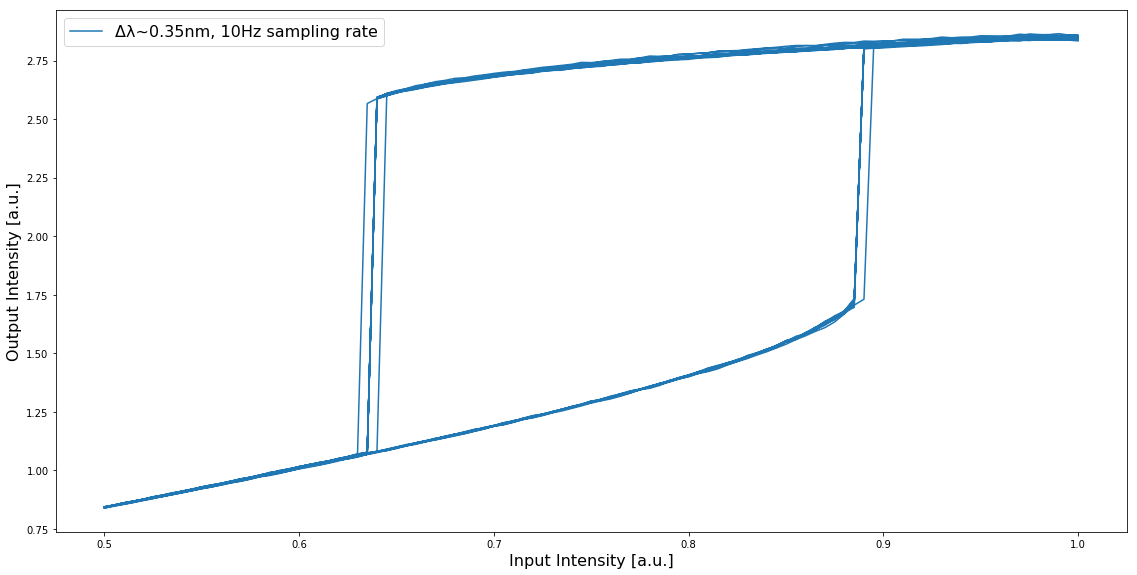
\includegraphics[draft,width=9cm,height=6cm]{figures/foo.png}
	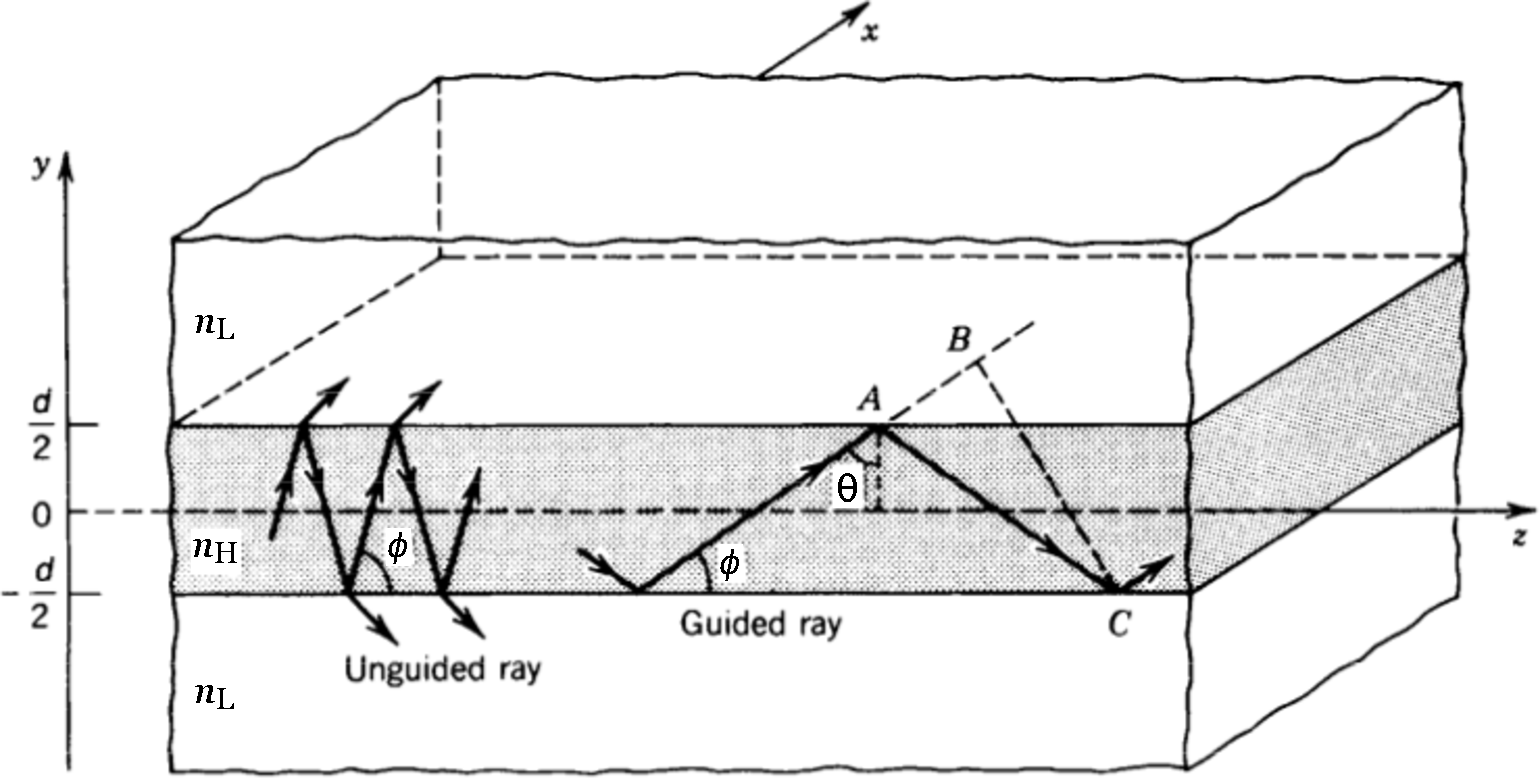
\includegraphics[scale=.4]{figures/dielBC.pdf}
	\caption{Scheme of a dielectric slab waveguide, made by two materials with refractive indexes $n_H$ and $n_L$.
		Two rays are shown: the unguided one is incident on the interface at an angle smaller than the critical angle.
		Conversely the guided ray is incident at an greater angle and is therefore totally reflected inside the waveguide \cite{Saleh1991}.}
	\label{fig:slabVG}
\end{figure}

2D-waveguides on the other hand are more common, to the point that with the term waveguide one usually refers to a device belonging to this category.
Since they confine light in two dimension, their core then becomes a straight path with which one can conduct light from a place to another.
A few types are shown in \autoref{fig:2DVG} below.

\begin{figure}[ht]
	\centering
%	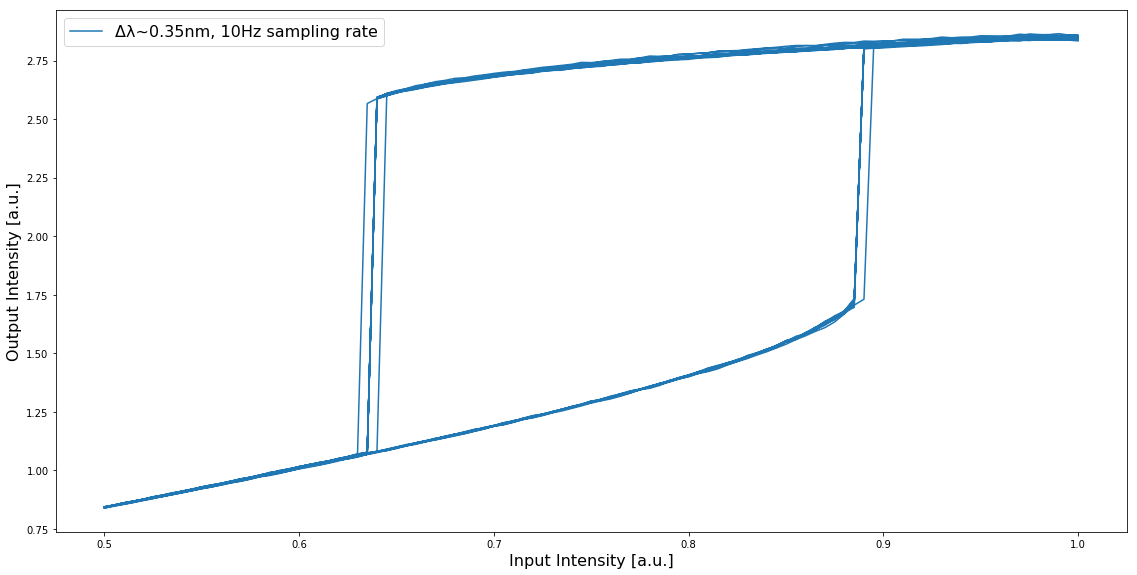
\includegraphics[draft,width=9cm,height=6cm]{figures/foo.png}
	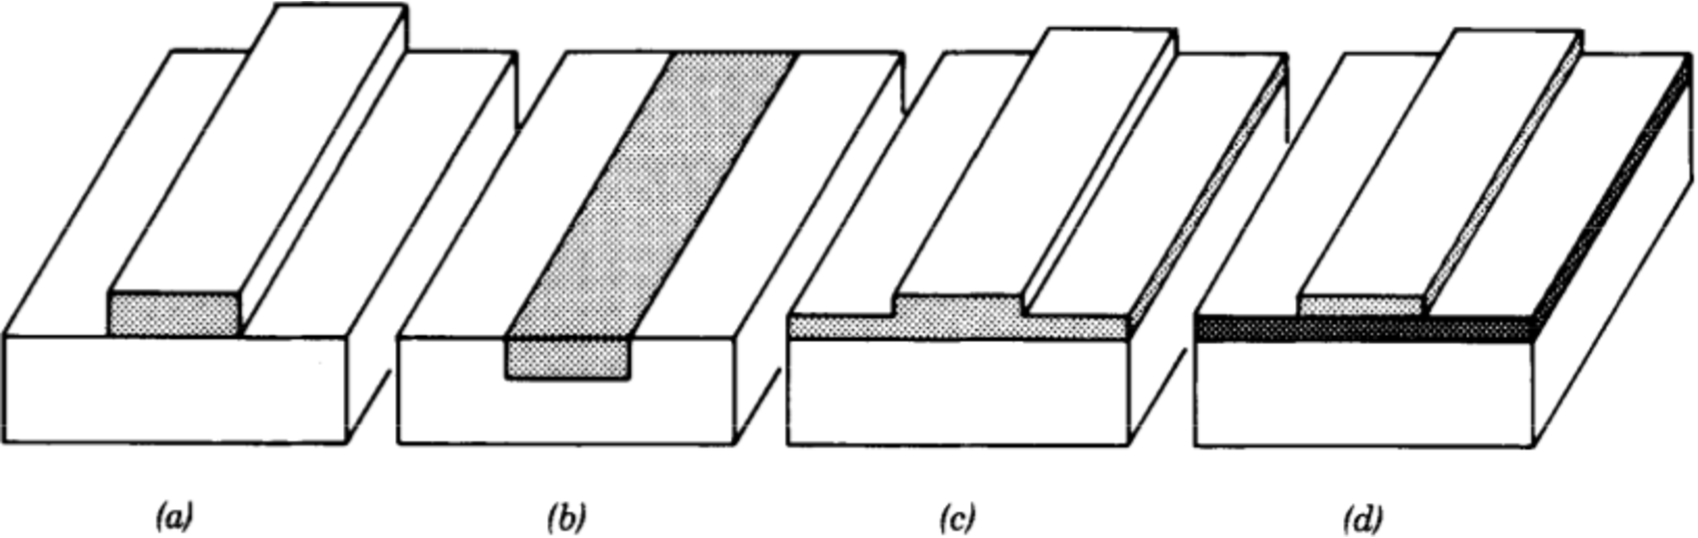
\includegraphics[scale=.4]{figures/WGtypes.pdf}
	\caption{Representation of a few types of 2D dielectric waveguides.
		Light is constrained in two direction and can only move forward or backward in the third direction.
		(a) strip, (b) embedded strip, (c) rib, (d) strip loaded \cite{Saleh1991}.
		}
	\label{fig:2DVG}
\end{figure}

Obviously, the versatility of straight (2D-) waveguides is limited.
Hence more complex structures such as bent waveguides have been developed.

\paragraph{Propagation of light inside waveguides\\}
\noindent Light propagates inside waveguides as superposition of transverse electro-magnetic (TEM) waves which keep reflecting on the interfaces of the core.
The result of the superposition is the so called \textit{mode}, which is expressed mathematically by
\begin{equation}
	\phi(\textbf{r}) = \phi_m\left( x, y \right) e^{i\left( \beta_m z - \omega t\right)}.
\end{equation}
$\phi_m\left( x, y \right)$ is the transverse field distribution, $z$ is the direction of propagation, $\beta_m$ is the propagation constant of the m-th mode, and $\omega=2\pi \ni$ is the angular frequency of light.
Each mode, identified by the $m$ idex, travels inside the waveguide with a certain propagation constant $\beta$ and maintaining a field distribution $\phi_m$.
Both of them depends on the materials and the geometry of the waveguide, however while $\beta_m$ decrease with increasing $m$ indexes, the features of the function $\phi_m$ grows in number.
Light either propagate in a manner described by a mode or superposition of modes or is rapidly scattered away.

The filed distribution of some of the first modes, in the simplest case of a slab waveguide, is represented in \autoref{fig:WGmodes} below.
\begin{figure}[ht]
	\centering
	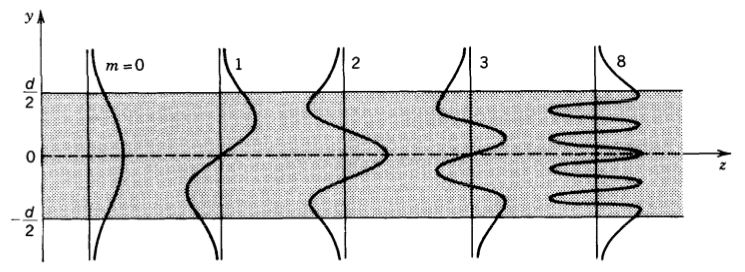
\includegraphics[scale=0.8]{figures/modes.png}
	\caption{Field distribution inside a slab waveguide.}
	\label{fig:WGmodes}
\end{figure}
The function inside the core is characterized by maxima, minima and nodes with a certain periodicity and the number of nodes (where the function is zero) is strictly linked to the index $m$.
Outside, the distribution of the field decays exponentially.
For waveguide with a 2D core, the field can be expected to be a multivariate version of the same or similar function.
However, differently from the analytical solution for slab waveguides, they are almost always found numerically.

The propagation constant can be written as
\begin{equation}
\beta_m = n_{eff} k_0
\end{equation}
where $k_0$ is the wavevector in vacuum and $n_{eff}$ is the \textit{effective refractive index} of the mode.
The value of this quantity is between the core refractive index and the cladding refractive index $n_L < n_{eff} < n_H$.
The physical interpretation of the effective index is that of an average refractive index \textit{felt} by the mode propagating as a whole, instead of a superposition of multiple TEM waves \textit{feeling} different refractive indexes depending on the specific medium in which they are propagating.
Similarly to the actual refractive index of materials, $n_{eff}$ is a complex number and the imaginary part is directly linked with the absorption properties of the materials.
Actually, a low imaginary part means that the material absorb less light and is therefore transparent.

All of these parameters which describe the propagation of light along the waveguide depends both on the materials and the geometry of the core and the cladding, but also on the frequency of light
For dielectric waveguides, the fundamental mode ($m=0$) is always supported while higher modes might or might not be, depending both on the waveguides and on the frequency of light.
For this reason one distinguish \textit{single-mode} waveguides, which allow propagation for only the fundamental mode in a certain operative range of frequencies, from \textit{multi-mode} waveguides, which allow higher order modes to propagate.

\subsection{Light coupling}
\label{ssec:light_coupling}
We covered how light travels inside a waveguide, now the problem on how to insert and extract light from it.
The process of inserting light into a waveguide is called \textit{coupling} and often requires to extract light at the same time from another waveguide.

\subsubsection{End coupling}
\label{sssec:end_coupling}
The most naive way to insert light into a waveguide is obviously to use one of its ends.
This is achieved either by radiating a beam directly on the whole waveguide or by focusing it inside the core with some lensing mechanism (e.g. tapered optical fibers).

These methods are very simple, however they have a low coupling efficiency. % and are only able to access structures at perimeter of a chip.

\subsubsection{Grating coupling}
\label{sssec:grating_coupling}
% and prism coupling?
A more sophisticated way to couple light inside a waveguide is to use the so called \textit{grating coupler}.
A grating coupler is a periodic structure end coupled to a waveguide.
It is designed in a way such that light incident from free space above it, at a certain angle and with a specific wavelength, is coupled inside the waveguide.

\subsubsection{Evanescent coupling}
\label{sssec:evanescent_coupling}
Evanescent coupling exploits the fact that the field distribution outside the core decays exponentially to zero.
This means that when two waveguides are separated by a sufficiently small distance, the field distribution of one waveguide cannot decays sufficiently fast to zero and instead extends itself over the core of the second waveguide.
When this happens optical power can be transferred between the waveguides.
Therefore, if at the beginning light is propagating inside one waveguide, light is \textit{coupled} inside the other waveguide because its mode overlaps the core of the second waveguide.
Depending on the parameters of the problems, light can couple completely or partially between the waveguides.

This exchange of optical power is periodic with their length.

\subsection{Microring Optical Cavity}
\label{ssec:Microring_Optical_Cavity}
In integrated photonics the microring is an optical cavity made by bending a waveguide on itself.
To insert light into the cavity, the microring is often side coupled with one or two straight waveguides.
Light inserted from the different ports into the cavity interfere with itself, after a round trip, and with each other.
When the waves are in phase, they generate constructive interference and the energy stored in the cavity increases exponentially.
On the other hand, when the signals are out of phase, the interference is destructive and the energy stored in the cavity remains low.

In the simpler case, when there is only one waveguide side coupled to the resonator, the optical cavity has only two ports, which are usually called \textit{input} and \textit{through}.
This configuration is called \textit{All-Pass Filter}, because in the ideal case, where no losses happen, all the signal passes from the input to the through channels.
%All pass filter theory\\
All pass resonators have only one input and one output: light enters the resonator from the input and exits from the output, unless the device is used backwards or some specific phenomena happens (e.g. back scattering).

%1.2.3.2 Add-drop filter theory\\
\subsubsection{Add-drop filter theory}
\label{sssec:Add-drop_filter_theory}
By adding a secondary couple of input and output ports, one obtains the so called add-drop resonator.
The name comes from the fact that the secondary input is used as an add port to convey additional content to the output channel, while the drop port is used to take some of the light from the input channel.
Of course, light might also travel from the input to the output and from the add to the drop.
Whether light goes straight or passes through the resonator depends on the frequency of the signals and the relative position of the resonance.
Resonators with more than four ports are possible, however are very uncommon.

\begin{figure}[ht]
	\centering
	\tikzsetexternalprefix{tikz/}	% set subfolder
\tikzsetnextfilename{ADF}
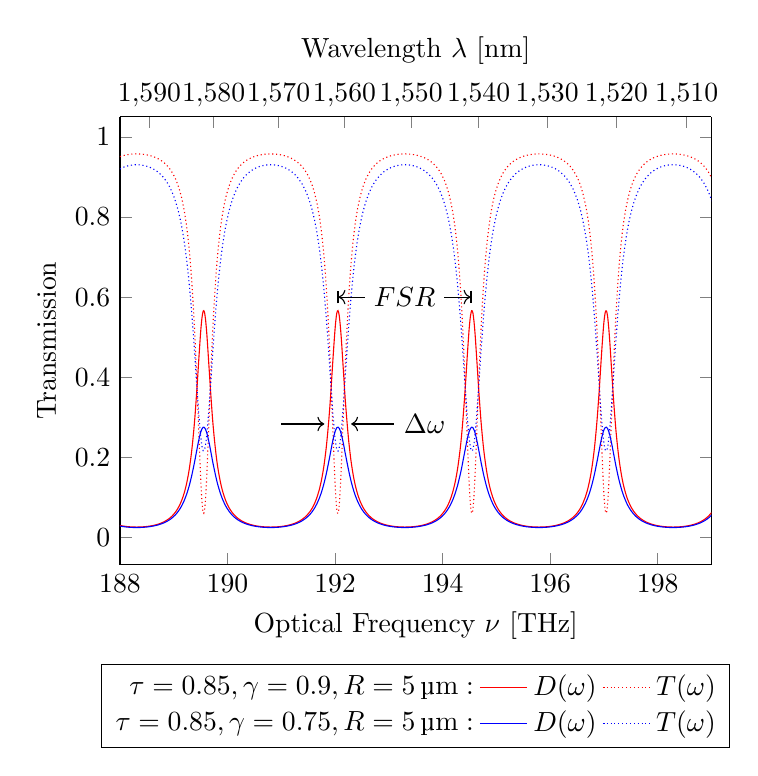
\begin{tikzpicture}
	\newcommand\CENTRAL{193}
	\newcommand\START{193-5}
	\newcommand\STOP {193+7}
	\newcommand\CC{299792458}
	
	\begin{axis}[%
			axis x line*= bottom,
%			scaled x ticks = manual:{$+\SI{193}{\THz}$}{ \pgfmathparse{#1-\CENTRAL} },%
			xlabel = {Optical Frequency $\nu$ [$\si{\THz}$]},
			ylabel = {Transmission},
			legend columns=3,
			legend cell align=right,
			legend style={ at={(0.5,-0.22)}, anchor=north },
			width=\textwidth*0.75,%
			height=207pt,
			xmin= 188, xmax = 199,
			%
			% global plot definition
			domain = \START:\STOP,
			samples = 551,
			smooth,
			no markers,
			cycle multi list={
%					exotic\nextlist 
					color list\nextlist
					solid,densely dotted
					%[2 of]linestyles
				},
			]
				
		\foreach \TA/\LA/\Radius/\Neff in {0.85/0.9/5/3.826, 0.85/0.75/5/3.826 }{ %, 0.9/0.99/5/3.826
			\edef\temp{
				\noexpand\addlegendimage{empty legend}
				\noexpand\addlegendentry{$\tau=\TA,\gamma=\LA,R=\SI{\Radius}{\um}:$};
				\noexpand\addplot 
										{ + (1-\TA^2)^2 * \LA
											/ ( (1-\TA^2 * \LA)^2 	+ 4 * \TA^2 	* \LA *sin(deg(\Neff*pi*\Radius*2*pi*x*1e6/\CC))^2 )
										};
				\noexpand\addlegendentry{$D(\omega)$};
				\noexpand\addplot 
										{ + \TA^2 * ( (1- \LA)^2	+ 4 					* \LA *sin(deg(\Neff*pi*\Radius*2*pi*x*1e6/\CC))^2 )
											/ ( (1-\TA^2 * \LA)^2 	+ 4 * \TA^2 	* \LA *sin(deg(\Neff*pi*\Radius*2*pi*x*1e6/\CC))^2 )
										};
				\noexpand\addlegendentry{$T(\omega)$};
								}
			\temp
		}
		
		\draw [|<->|] (192.0446013229, 0.6) -- (194.5386870543, 0.6) node [midway, fill=white] {$FSR$};%0.5665693
	
		\draw [<-] (192.3, 0.283) -- (193.1,0.283) node [right] {$\Delta\omega$}; %0.5665693/2 = 0.283
		\draw [<-] (191.8, 0.283) -- (191,0.283) {};	
		
	\end{axis}
	
	\begin{axis}[
			width=\textwidth*0.75,%
			height=207pt,
			axis x line*= top,
			axis y line = none,
			xlabel = {Wavelength $\lambda$ [\si{\nm}]},
			xmin= 188, xmax = 199,
%			xmin= 150, xmax = 250,
%  		xtick = {187.37029,188.54872,189.74206,190.95061,192.17465,193.41449,194.67043,195.94278,197.23188,198.53805,199.86163},
			xtick = {187.37029,188.54872,189.74206,190.95061,192.17465,193.4143 ,194.67043,195.94278,197.2318 ,198.53805,199.86163},
%			xtick = {157.785504211, 171.309976, 187.37029, 199.86163, 214.13747, 230.609583077, 249.827048333},
%			scaled x ticks = manual:{$+\SI{1500}{\nm}$}{ \pgfkeys{/pgf/fpu}\pgfmathparse{(1e-3*\CC/#1) - 1500} },
			scaled x ticks = manual:{}{ \pgfkeys{/pgf/fpu}\pgfmathparse{(1e-3*\CC/#1)} },
		]
		\addplot[black, opacity=0, domain = \START:\STOP] {0}; %
	\end{axis}
\end{tikzpicture}
	\caption{Transmission spectra of microring resonators in Add-Drop Filter configuration for the through and drop ports.}
	\label{fig:ADF}
\end{figure}

\subsection{Nonlinear Perturbations}
\label{ssec:Nonlinear_Perturbations}

Comparison between nonlinear optics phenomena which affect a microring dynamic:
\begin{itemize}
\item TOC
\item FCD
\item FCA
\item Kerr
\item TPA
\end{itemize}

\section{Integrated photonics applied to ANNs}
\label{sec:Integrated_photonics_applied_to_ANNs}
Since our experiments are carried out in a time scale such that physics phenomena can be considered quasi-static, we obtain also that the only nonlinear effect non negligible is the thermo-optic effect.

\subsection{Weighted sum of inputs}
\label{ssec:Weighted_Sum_of_inputs}
This has already been demonstrated and integrated widely, so it will not be the focus of this work.
Two example are the banks of microring resonators and the MZ interferometers.

\subsection{Nonlinear Activation Function}
\label{ssec:Nonlinear_Activation_Function}
As opposed to the mechanism for weighted sum, an optical phenomenon for the activation function in an integrated photonic circuit has yet to be proposed.

\subsection{Simulations}
\label{ssec:Simulations}

\begin{figure}[ht]
	\centering
	\tikzsetexternalprefix{tikz/}	% set subfolder
\tikzsetnextfilename{bistability_test}
% This file was created by matplotlib2tikz v0.6.15.
\begin{tikzpicture}[baseline]
	
	\pgfplotstableread[col sep=tab, header=true]{tikz/foo.csv}\loadedtable
	
	\pgfplotstablegetcolsof{\loadedtable}
	\pgfmathparse{\pgfplotsretval - 1}
	\newcommand{\ncol}{\pgfmathresult}
	
	\definecolor{color1}{rgb}{1,0.498039215686275,0.0549019607843137}
	\definecolor{color6}{rgb}{0.890196078431372,0.466666666666667,0.76078431372549}
	\definecolor{color5}{rgb}{0.549019607843137,0.337254901960784,0.294117647058824}
	\definecolor{color2}{rgb}{0.172549019607843,0.627450980392157,0.172549019607843}
	\definecolor{color4}{rgb}{0.580392156862745,0.403921568627451,0.741176470588235}
	\definecolor{color3}{rgb}{0.83921568627451,0.152941176470588,0.156862745098039}
	\definecolor{color0}{rgb}{0.12156862745098,0.466666666666667,0.705882352941177}

\begin{axis}[
		title={Internal Power},
		xlabel={Pump Power $P$ $[mW]$},
		ylabel={Internal Power [a.u.*]},
		xmin=0.852408771935031, xmax=4.09941578936435,
		ymin=-3215.6821653405, ymax=90671.1511338174,
		tick align=outside,
		tick pos=left,
		width=\textwidth*0.75,%
		height=207pt,
		%x grid style={lightgray!92.02614379084967!black},
		%y grid style={lightgray!92.02614379084967!black},
		legend entries={
			{$\Delta\lambda$},
			{\SI{350}{\pm}},
			{\SI{379}{\pm}},
			{\SI{407}{\pm}},
			{\SI{436}{\pm}},
			{\SI{464}{\pm}},
			{\SI{493}{\pm}},
			{\SI{521}{\pm}},
			{\SI{550}{\pm}}
			},
		legend pos = outer north east,
		%legend cell align={left},
		%legend style={at={(1,-0.1)}, anchor=north west, draw=white!80.0!black},
		%legend columns=8
	]
	
	\addlegendimage{empty legend}
	\addlegendimage{mark=*, color0}
	\addlegendimage{mark=*, color1}
	\addlegendimage{mark=*, color2}
	\addlegendimage{mark=*, color3}
	\addlegendimage{mark=*, color4}
	\addlegendimage{mark=*, color5}
	\addlegendimage{mark=*, color6}
	\addlegendimage{mark=*, gray!99.6078431372549!black}

%\addlegendentry = {$\Delta\lambda$}
%\addlegendimage = {empty legend}
%\foreach \i in {1,2...,\pgfplotsretval-1} {
%	\addplot table [x index=0, y index=\i] {\loadedtable};
%	\pgfplotstablegetcolumnnamebyindex{\i}\of{\loadedtable}\to\colname
%	\addlegendentry = {\SI{\colname}{\pm}}
%	\addlegendimage = {mark=*, color\i}
%}

\addplot [semithick, color0, mark=*, mark size=1, mark options={solid}]
table {%
1 2182.13784798453
1.10996151344182 2732.06812562319
1.20997071148193 3301.35802903992
1.30232241935941 3891.75515464847
1.38854537026638 4505.26943967214
1.46971861477299 5144.22980210166
1.54663743906977 5811.35713826561
1.61990800024395 6509.85972553239
1.69000487886171 7243.55987029429
1.75730789900303 8017.0649998584
1.82212667320922 8836.00339261668
1.88471753176505 9707.35631717665
1.94529553946556 10639.9381155571
2.00404323735458 11645.110858216
2.06111713847338 12737.8851497554
2.11665264505793 13938.6847549387
2.1707678321628 15276.31091276
2.22356640163383 16793.2014266478
2.27514001850367 18555.3533357662
2.32557018064795 20672.1913566021
2.37492973084278 23336.6084050299
2.42328409142697 26875.9830526321
2.47069228134243 31476.9310455102
2.51720776067593 36046.2694806532
2.56287913716765 39544.1852080518
2.60775076129818 42181.9936544263
2.65186323070653 44282.0696014857
2.69525382027284 46032.9554507758
2.73795685083191 47541.7982041075
2.78000400689269 48873.3912118438
2.82142461172746 50069.4947595316
2.86224586662004 51158.5039921599
2.9024930598204 52160.5856929643
2.94218974976591 53090.5802810476
2.98135792633989 53959.7327474007
3.02001815330168 54776.7742586017
3.05818969450781 55548.625360946
3.09589062612293 56280.8689540435
3.13313793667592 56978.0778524274
3.16994761653247 57644.0474967912
3.20633473812108 58281.9649496754
3.24231352805431 58894.5341847922
3.27789743212414 59484.0704107321
3.31309917401337 60052.5723212442
3.34793080845022 60601.7782354623
3.38240376943561 61133.2101736674
3.41652891409018 61648.2089375426
3.45031656259774 62147.9622831466
3.48377653466154 62633.5277873525
3.51691818283855 63105.8515562808
3.54975042307237 63565.7836494865
3.58228176270719 64014.090916815
3.61452032623231 64451.4677214149
3.64647387897796 64878.5449862339
3.67814984895812 65295.8978439847
3.70955534703456 65704.052169585
3.74069718555709 66103.4901635271
3.77158189561844 66494.655157941
3.80221574304758 66877.9557805134
3.83260474325241 67253.7695572549
3.86275467501147 67622.4460626382
3.89267109330405 67984.3096727404
3.92235934125968 68339.6619855259
3.95182456129939 68688.7839488388
};
\addplot [semithick, color1, mark=*, mark size=1, mark options={solid}]
table {%
1 1940.07544411095
1.10996151344182 2423.22716305164
1.20997071148193 2920.70721201128
1.30232241935941 3433.61186262683
1.38854537026638 3963.17696183345
1.46971861477299 4510.8034528873
1.54663743906977 5078.08911859356
1.61990800024395 5666.86848769019
1.69000487886171 6279.26358787269
1.75730789900303 6917.74933289089
1.82212667320922 7585.2389829278
1.88471753176505 8285.19764576196
1.94529553946556 9021.7957820453
2.00404323735458 9800.12113436134
2.06111713847338 10626.4782986138
2.11665264505793 11508.8239192492
2.1707678321628 12457.4194811703
2.22356640163383 13485.848418119
2.27514001850367 14612.6752996465
2.32557018064795 15864.3096818447
2.37492973084278 17280.3143272715
2.42328409142697 18924.1988617378
2.47069228134243 20908.2895226999
2.51720776067593 23462.0392880969
2.56287913716765 27170.8381037511
2.60775076129818 33631.0297137638
2.65186323070653 40341.9479641702
2.69525382027284 44189.4013634534
2.73795685083191 46803.6856546889
2.78000400689269 48821.2416782276
2.82142461172746 50486.4792493101
2.86224586662004 51917.3882993097
2.9024930598204 53180.0763622241
2.94218974976591 54315.4654194578
2.98135792633989 55350.7465285369
3.02001815330168 56304.9665061537
3.05818969450781 57192.0231155222
3.09589062612293 58022.3918927019
3.13313793667592 58804.1805477364
3.16994761653247 59543.8034465492
3.20633473812108 60246.430206525
3.24231352805431 60916.2935960542
3.27789743212414 61556.9070656952
3.31309917401337 62171.2219851855
3.34793080845022 62761.7437447084
3.38240376943561 63330.6190515937
3.41652891409018 63879.7026494471
3.45031656259774 64410.6090421554
3.48377653466154 64924.7531439948
3.51691818283855 65423.3825577898
3.54975042307237 65907.6035338806
3.58228176270719 66378.4020054886
3.61452032623231 66836.6608209025
3.64647387897796 67283.1739473754
3.67814984895812 67718.6582859319
3.70955534703456 68143.7635642359
3.74069718555709 68559.0806667746
3.77158189561844 68965.1487014138
3.80221574304758 69362.4610174769
3.83260474325241 69751.4703637162
3.86275467501147 70132.5933346228
3.89267109330405 70506.2142143482
3.92235934125968 70872.6883067225
3.95182456129939 71232.3448615192
};
\addplot [semithick, color2, mark=*, mark size=1, mark options={solid}]
table {%
1 1732.97280209881
1.10996151344182 2160.25082035293
1.20997071148193 2598.25542831804
1.30232241935941 3047.68385058352
1.38854537026638 3509.3086372655
1.46971861477299 3983.98931489536
1.54663743906977 4472.68642687737
1.61990800024395 4976.47859191022
1.69000487886171 5496.5834020755
1.75730789900303 6034.38326074926
1.82212667320922 6591.45765894542
1.88471753176505 7169.62394084324
1.94529553946556 7770.98943472775
2.00404323735458 8398.01903253042
2.06111713847338 9053.62415924678
2.11665264505793 9741.28193834583
2.1707678321628 10465.1979664045
2.22356640163383 11230.5337188335
2.27514001850367 12043.7326151105
2.32557018064795 12913.002021987
2.37492973084278 13849.0520482085
2.42328409142697 14866.2785935804
2.47069228134243 15984.7629825415
2.51720776067593 17233.8916436386
2.56287913716765 18659.5263921909
2.60775076129818 20340.0938776341
2.65186323070653 22430.0792057072
2.69525382027284 25321.8960673326
2.73795685083191 30987.8016123129
2.78000400689269 44888.9927766667
2.82142461172746 48918.4586028915
2.86224586662004 51428.5184753255
2.9024930598204 53337.2501195886
2.94218974976591 54909.1358036994
2.98135792633989 56261.2528516411
3.02001815330168 57456.8190350748
3.05818969450781 58534.2614456403
3.09589062612293 59518.8696435552
3.13313793667592 60428.26786974
3.16994761653247 61275.282136951
3.20633473812108 62069.5689773745
3.24231352805431 62818.6003117727
3.27789743212414 63528.2893700834
3.31309917401337 64203.4049985116
3.34793080845022 64847.8553330121
3.38240376943561 65464.8876903212
3.41652891409018 66057.2328970549
3.45031656259774 66627.2118303121
3.48377653466154 67176.8154208414
3.51691818283855 67707.7658504522
3.54975042307237 68221.5639803765
3.58228176270719 68719.5266349635
3.61452032623231 69202.8162397473
3.64647387897796 69672.4646422314
3.67814984895812 70129.3924540031
3.70955534703456 70574.4248816071
3.74069718555709 71008.3048010219
3.77158189561844 71431.7036445875
3.80221574304758 71845.2304972518
3.83260474325241 72249.4397994264
3.86275467501147 72644.8378492904
3.89267109330405 73031.8883777777
3.92235934125968 73411.0173027476
3.95182456129939 73782.6168527726
};
\addplot [semithick, color3, mark=*, mark size=1, mark options={solid}]
table {%
1 1555.12712962575
1.10996151344182 1935.35022328765
1.20997071148193 2323.70064537386
1.30232241935941 2720.62917693881
1.38854537026638 3126.62808241723
1.46971861477299 3542.23655447464
1.54663743906977 3968.04710570885
1.61990800024395 4404.71310972971
1.69000487886171 4852.95775950785
1.75730789900303 5313.58477279263
1.82212667320922 5787.49128427383
1.88471753176505 6275.68348806087
1.94529553946556 6779.2957771205
2.00404323735458 7299.61438270963
2.06111713847338 7838.1068655017
2.11665264505793 8396.45931641251
2.1707678321628 8976.62387064854
2.22356640163383 9580.88022625359
2.27514001850367 10211.916530394
2.32557018064795 10872.9375886795
2.37492973084278 11567.812506292
2.42328409142697 12301.2807338782
2.47069228134243 13079.2472517646
2.51720776067593 13909.2186734183
2.56287913716765 14800.9715720034
2.60775076129818 15767.623259535
2.65186323070653 16827.4446215626
2.69525382027284 18007.1530903572
2.73795685083191 19348.4800019746
2.78000400689269 20923.1011850703
2.82142461172746 22874.1137116357
2.86224586662004 25581.679254139
2.9024930598204 32373.8833560084
2.94218974976591 53685.3764633791
2.98135792633989 56034.1288896655
3.02001815330168 57820.9838468359
3.05818969450781 59297.9114358345
3.09589062612293 60573.1864351054
3.13313793667592 61704.6888586915
3.16994761653247 62727.4816976698
3.20633473812108 63664.6266831185
3.24231352805431 64532.2068880532
3.27789743212414 65341.9425439077
3.31309917401337 66102.6722811745
3.34793080845022 66821.2474128613
3.38240376943561 67503.0999560958
3.41652891409018 68152.6186366019
3.45031656259774 68773.406464817
3.48377653466154 69368.4623655541
3.51691818283855 69940.3124659625
3.54975042307237 70491.1070517066
3.58228176270719 71022.6935267439
3.61452032623231 71536.6722322788
3.64647387897796 72034.4397820577
3.67814984895812 72517.2231554371
3.70955534703456 72986.1068373264
3.74069718555709 73442.0546571947
3.77158189561844 73885.9275378199
3.80221574304758 74318.4980334294
3.83260474325241 74740.4623689852
3.86275467501147 75152.4504450848
3.89267109330405 75555.034238381
3.92235934125968 75948.7348944082
3.95182456129939 76334.028743014
};
\addplot [semithick, color4, mark=*, mark size=1, mark options={solid}]
table {%
1 1401.7392420467
1.10996151344182 1742.05447923165
1.20997071148193 2088.60129970629
1.30232241935941 2441.67621144985
1.38854537026638 2801.59908560004
1.46971861477299 3168.71577477143
1.54663743906977 3543.40111578359
1.61990800024395 3926.06239167527
1.69000487886171 4317.14333702743
1.75730789900303 4717.12879862109
1.82212667320922 5126.55018167644
1.88471753176505 5545.99185421269
1.94529553946556 5976.0987168996
2.00404323735458 6417.58521344896
2.06111713847338 6871.24612225125
2.11665264505793 7337.96958510755
2.1707678321628 7818.75295467511
2.22356640163383 8314.72224806523
2.27514001850367 8827.15625233288
2.32557018064795 9357.51670762848
2.37492973084278 9907.48654853509
2.42328409142697 10479.0189765846
2.47069228134243 11074.4013469418
2.51720776067593 11696.3396961176
2.56287913716765 12348.0726453624
2.60775076129818 13033.5281305727
2.65186323070653 13757.5443237197
2.69525382027284 14526.1899146087
2.73795685083191 15347.2441508942
2.78000400689269 16230.9456576159
2.82142461172746 17191.2192207557
2.86224586662004 18247.8134492887
2.9024930598204 19430.3365989971
2.94218974976591 20786.7549552248
2.98135792633989 22404.3765552702
3.02001815330168 24477.132776658
3.05818969450781 27686.4341351164
3.09589062612293 60604.7367382226
3.13313793667592 62267.3306556756
3.16994761653247 63651.8767800161
3.20633473812108 64854.0003360527
3.24231352805431 65925.1989624745
3.27789743212414 66896.8638024415
3.31309917401337 67789.7512506825
3.34793080845022 68618.4032399159
3.38240376943561 69393.4596711254
3.41652891409018 70122.9731701597
3.45031656259774 70813.2057695201
3.48377653466154 71469.1366375532
3.51691818283855 72094.7992028596
3.54975042307237 72693.5127477348
3.58228176270719 73268.04615849
3.61452032623231 73820.7365353523
3.64647387897796 74353.577049637
3.67814984895812 74868.2831356681
3.70955534703456 75366.343267635
3.74069718555709 75849.0584399384
3.77158189561844 76317.5732904656
3.80221574304758 76772.9009091922
3.83260474325241 77215.9428404241
3.86275467501147 77647.5053551995
3.89267109330405 78068.3128118444
3.92235934125968 78479.018719511
3.95182456129939 78880.2149507901
};
\addplot [semithick, color5, mark=*, mark size=1, mark options={solid}]
table {%
1 1268.82868775917
1.10996151344182 1575.05802024631
1.20997071148193 1886.12026197023
1.30232241935941 2202.21379773944
1.38854537026638 2523.5504741739
1.46971861477299 2850.35689401489
1.54663743906977 3182.87587513696
1.61990800024395 3521.36809814379
1.69000487886171 3866.11397301945
1.75730789900303 4217.4157647887
1.82212667320922 4575.60001730141
1.88471753176505 4941.02033443108
1.94529553946556 5314.06057831588
2.00404323735458 5695.1385694657
2.06111713847338 6084.71038352431
2.11665264505793 6483.27536643047
2.1707678321628 6891.38202520844
2.22356640163383 7309.63497755628
2.27514001850367 7738.70321414165
2.32557018064795 8179.32997495534
2.37492973084278 8632.34465296927
2.42328409142697 9098.67724862147
2.47069228134243 9579.37607223338
2.51720776067593 10075.6296358352
2.56287913716765 10588.794003145
2.60775076129818 11120.4273476226
2.65186323070653 11672.3341837221
2.69525382027284 12246.6227764755
2.73795685083191 12845.7808515076
2.78000400689269 13472.7772471925
2.82142461172746 14131.2012233633
2.86224586662004 14825.4579311768
2.9024930598204 15561.0503423298
2.94218974976591 16344.9992760867
2.98135792633989 17186.4940437196
3.02001815330168 18097.9494922264
3.05818969450781 19096.8290326469
3.09589062612293 20209.0416065191
3.13313793667592 21475.970206772
3.16994761653247 22971.3891448233
3.20633473812108 24853.4294810608
3.24231352805431 27628.5741492578
3.27789743212414 67971.5517060323
3.31309917401337 69105.1416733301
3.34793080845022 70120.0946247003
3.38240376943561 71044.1745834219
3.41652891409018 71895.906585186
3.45031656259774 72688.3618266287
3.48377653466154 73431.1596717701
3.51691818283855 74131.6157929157
3.54975042307237 74795.4428143908
3.58228176270719 75427.1994959916
3.61452032623231 76030.5904912877
3.64647387897796 76608.6731994837
3.67814984895812 77164.0045519713
3.70955534703456 77698.7477761974
3.74069718555709 78214.7516479251
3.77158189561844 78713.6104264719
3.80221574304758 79196.7099098472
3.83260474325241 79665.2633847461
3.86275467501147 80120.339956786
3.89267109330405 80562.8872403561
3.92235934125968 80993.7496498591
3.95182456129939 81413.6833305709
};
\addplot [semithick, color6, mark=*, mark size=1, mark options={solid}]
table {%
1 1153.11534113191
1.10996151344182 1430.03226695262
1.20997071148193 1710.73804990963
1.30232241935941 1995.36761972763
1.38854537026638 2284.06383596786
1.46971861477299 2576.97814784539
1.54663743906977 2874.271324898
1.61990800024395 3176.11426828301
1.69000487886171 3482.68891680214
1.75730789900303 3794.18925621961
1.82212667320922 4110.82245204988
1.88471753176505 4432.81012075285
1.94529553946556 4760.38976134927
2.00404323735458 5093.81637550133
2.06111713847338 5433.36430322558
2.11665264505793 5779.32931126422
2.1707678321628 6132.03098200405
2.22356640163383 6491.81544913815
2.27514001850367 6859.0585527477
2.32557018064795 7234.16948577099
2.37492973084278 7617.59503665301
2.42328409142697 8009.82454518515
2.47069228134243 8411.39572435789
2.51720776067593 8822.9015440492
2.56287913716765 9244.9984176772
2.60775076129818 9678.41600447315
2.65186323070653 10123.9690407346
2.69525382027284 10582.5717252035
2.73795685083191 11055.255374458
2.78000400689269 11543.1902961492
2.82142461172746 12047.7131731641
2.86224586662004 12570.3617592033
2.9024930598204 13112.9194050828
2.94218974976591 13677.4730410114
2.98135792633989 14266.4899249147
3.02001815330168 14882.92113088
3.05818969450781 15530.3440849035
3.09589062612293 16213.1637448906
3.13313793667592 16936.9048102428
3.16994761653247 17708.6507936515
3.20633473812108 18537.731333299
3.24231352805431 19436.8536726255
3.27789743212414 20424.0877878307
3.31309917401337 21526.6517346132
3.34793080845022 22789.0048056135
3.38240376943561 24293.3410848102
3.41652891409018 26228.6066943418
3.45031656259774 29348.8257048927
3.48377653466154 75171.1397221552
3.51691818283855 75984.6568808932
3.54975042307237 76743.4666071406
3.58228176270719 77456.2449920176
3.61452032623231 78129.6279619962
3.64647387897796 78768.8222956222
3.67814984895812 79377.9997469359
3.70955534703456 79960.5631547749
3.74069718555709 80519.3292809379
3.77158189561844 81056.6605048151
3.80221574304758 81574.5604661358
3.83260474325241 82074.7454388648
3.86275467501147 82558.6984882122
3.89267109330405 83027.7111994293
3.92235934125968 83482.9163354476
3.95182456129939 83925.3136700693
};
\addplot [semithick, gray!99.6078431372549!black, mark=*, mark size=1, mark options={solid}]
table {%
1 1051.90116643941
1.10996151344182 1303.44726288011
1.20997071148193 1557.99394172329
1.30232241935941 1815.63441347309
1.38854537026638 2076.46666063304
1.46971861477299 2340.59378187961
1.54663743906977 2608.12436994593
1.61990800024395 2879.17292492343
1.69000487886171 3153.86030778706
1.75730789900303 3432.31424093356
1.82212667320922 3714.66985891778
1.88471753176505 4001.07031664975
1.94529553946556 4291.66746463481
2.00404323735458 4586.622597123
2.06111713847338 4886.1072842512
2.11665264505793 5190.30430224765
2.1707678321628 5499.40867237775
2.22356640163383 5813.62882592496
2.27514001850367 6133.18791706005
2.32557018064795 6458.32530267821
2.37492973084278 6789.29821739155
2.42328409142697 7126.38367974316
2.47069228134243 7469.88066200891
2.51720776067593 7820.1125779211
2.56287913716765 8177.43014050562
2.60775076129818 8542.21466092436
2.65186323070653 8914.88187908926
2.69525382027284 9295.88642441276
2.73795685083191 9685.72704972988
2.78000400689269 10084.9527957754
2.82142461172746 10494.1703087648
2.86224586662004 10914.0525718883
2.9024930598204 11345.3494129332
2.94218974976591 11788.9002336084
2.98135792633989 12245.6495758424
3.02001815330168 12716.6663249425
3.05818969450781 13203.1676488722
3.09589062612293 13706.549171899
3.13313793667592 14228.4234937297
3.16994761653247 14770.6700428606
3.20633473812108 15335.5006187596
3.24231352805431 15925.5470950771
3.27789743212414 16543.9811598262
3.31309917401337 17194.6816380418
3.34793080845022 17882.4746784895
3.38240376943561 18613.4896944253
3.41652891409018 19395.7073085347
3.45031656259774 20239.8430326763
3.48377653466154 21160.8577524495
3.51691818283855 22180.7408622233
3.54975042307237 23334.1838011124
3.58228176270719 24681.9491843409
3.61452032623231 26350.5329837158
3.64647387897796 28717.9644245379
3.67814984895812 81469.8024553932
3.70955534703456 82117.9322483101
3.74069718555709 82734.115466073
3.77158189561844 83322.1707454383
3.80221574304758 83885.2242523683
3.83260474325241 84425.872718139
3.86275467501147 84946.3003285067
3.89267109330405 85448.3644825201
3.92235934125968 85933.6599597318
3.95182456129939 86403.5678020375
};
\end{axis}

\end{tikzpicture}
	\caption{}
%	\label{fig:bist_test}
\end{figure}

\begin{figure}[ht]
	\centering
	\tikzsetexternalprefix{tikz/}	% set subfolder
\tikzsetnextfilename{bistability_test2}
% This file was created by matplotlib2tikz v0.6.15.

\newcommand{\downfile}[1]{
    \pgfplotstableread[col sep=tab, header=true]{#1}{\table}
    \pgfplotstablegetcolsof{#1}
    \pgfmathtruncatemacro\numberofcols{\pgfplotsretval - 1}
    \pgfplotsinvokeforeach{1,...,\numberofcols}{
        \pgfplotstablegetcolumnnamebyindex{##1}\of{\table}\to{\colname}
        \addplot [name path=down##1, semithick, color##1, mark=*, mark size=1, mark options={solid}]%
        		table [x index= 0, y index=##1] {#1};
        \addlegendentryexpanded{ \colname }
    }
}

\newcommand{\upfile}[1]{
    \pgfplotstableread[col sep=tab, header=true]{#1}{\table}
    \pgfplotstablegetcolsof{#1}
    \pgfmathtruncatemacro\numberofcols{\pgfplotsretval - 1}
    \pgfplotsinvokeforeach{1,...,\numberofcols}{
        \pgfplotstablegetcolumnnamebyindex{##1}\of{\table}\to{\colname}
        \addplot [name path=up##1, semithick, color##1, mark=*, mark size=1, mark options={solid}]%
        		table [x index= 0, y index=##1] {#1};
    }
}

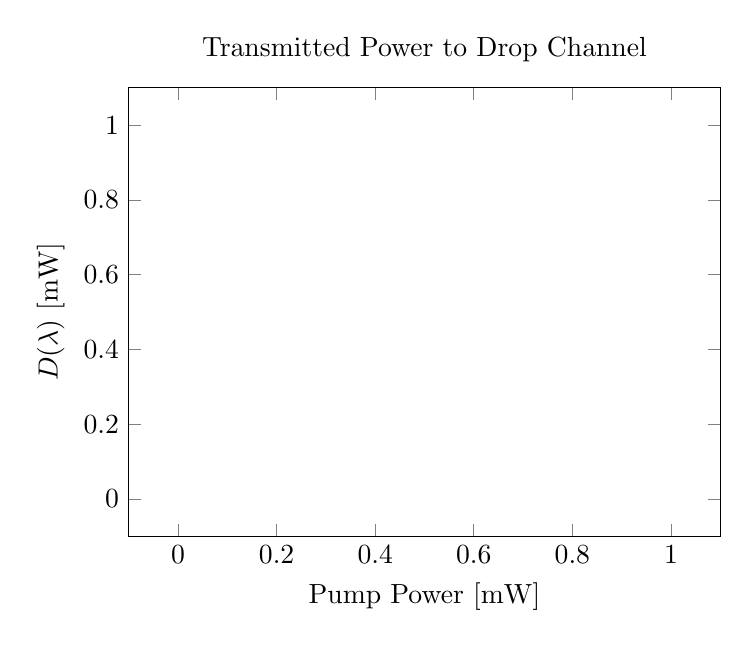
\begin{tikzpicture}[baseline]

	\definecolor{color1}{rgb}{0.12156862745098,0.466666666666667,0.705882352941177}
	\definecolor{color2}{rgb}{1,0.498039215686275,0.0549019607843137}
	\definecolor{color3}{rgb}{0.172549019607843,0.627450980392157,0.172549019607843}
	\definecolor{color4}{rgb}{0.83921568627451,0.152941176470588,0.156862745098039}
	\definecolor{color5}{rgb}{0.580392156862745,0.403921568627451,0.741176470588235}
	\definecolor{color6}{rgb}{0.549019607843137,0.337254901960784,0.294117647058824}
	\definecolor{color7}{rgb}{0.890196078431372,0.466666666666667,0.76078431372549}
	\definecolor{color8}{rgb}{0.45,0.45,0.45}
	\definecolor{color9}{rgb}{0.25,0.25,0.99}
	
	\begin{axis}[
			title={Transmitted Power to Drop Channel},
			xlabel={Pump Power [\si{mW}]},
			ylabel={$D(\lambda)$ [\si{\mW}]},
%			tick align=outside,
%			tick pos=left,
			width=\textwidth*0.75,%
			height=207pt,
			legend pos = outer north east,
			%cycle list name=color list,
			forget plot style={opacity=0.4},
		]
		\addlegendentry{\hspace{-.6cm}$\Delta\lambda$ in \si{\pm}}
		\addlegendimage{empty legend};
		
		\upfile{tikz/upwards.csv}
		\downfile{tikz/downwards.csv}

    \addplot [fill=color1, opacity=0.2] fill between [of=up1 and down1];
    \addplot [fill=color2, opacity=0.2] fill between [of=up2 and down2];
    \addplot [fill=color3, opacity=0.2] fill between [of=up3 and down3];
    \addplot [fill=color4, opacity=0.2] fill between [of=up4 and down4];
    \addplot [fill=color5, opacity=0.2] fill between [of=up5 and down5];
    \addplot [fill=color6, opacity=0.2] fill between [of=up6 and down6];
    \addplot [fill=color7, opacity=0.2] fill between [of=up7 and down7];
    \addplot [fill=color8, opacity=0.2] fill between [of=up8 and down8];
    \addplot [fill=color9, opacity=0.2] fill between [of=up9 and down9];
	\end{axis}
\end{tikzpicture}
	\caption{}
%	\label{fig:bist_test}
\end{figure}

% third chapter "Samples, setup and measurements" ~ 20pg
\chapter{Samples, setup and experiments}
\label{ch:experiments}

All the experiments have been made on samples manufactured for the IRIS project.
This is due to the fact that in the time frame of this work there would have not been enough time to design and produce an ad hoc device.
Moreover, as already stated, the aim of this thesis is to produce a proof of concept for an all-optical implementation of an activation function, rather than to construct a complete prototype.

\section{The samples}
%The samples used in this work have been provided by the IRIS project.
The IRIS project studied the design and the implementation of an integrated reconfigurable silicon photonics switch matrix, a routing device, as a replacement for electronic devices used in the telecommunication industry.
The completed integrated photonic circuit consists of a matrix of waveguides crossing each other and linked by couples of racetrack resonators, thermally-controlled.
At the ends of the waveguides other structures, interleavers and AWGs, allowed many signals at different wavelengths to be multiplexed/demultiplexed on/from the same waveguide.

The complexity of such photonic circuit required the fabrication, for testing purposes, of each and every structure of which it is composed, with various production parameters.
The collection of all these devices on a chip was produced in many samples.
Isolated from the others, but also grouped together with few other elements.
Specifically these test structures were disposed on a single chip and were accessible via grating couplers.


Since this work is at the beginning of the project, my choice was a system of intermediate complexity, so that it could be used both to test the activation function and the weighted sum.

The structure selected is the following: a simple waveguide, coupled to eight drop channels by a single or a couple of ring resonators each, nicknamed \textit{mini-matrix}.
In this family of devices, there were those built with single microrings, double microrings, single racetracks, or double racetracks.
The final choice was to study the \textit{mini-matrix} in which the coupling mechanism was provided by single ring resonators, because of its simpler transfer function in respect to double microrings or double racetracks.

Moreover, these samples were manufactured with thermo-electric \ref{this is not the correct term} pads to heat the rings and effectively tune their resonance.

\begin{figure}[ht]
	\centering
	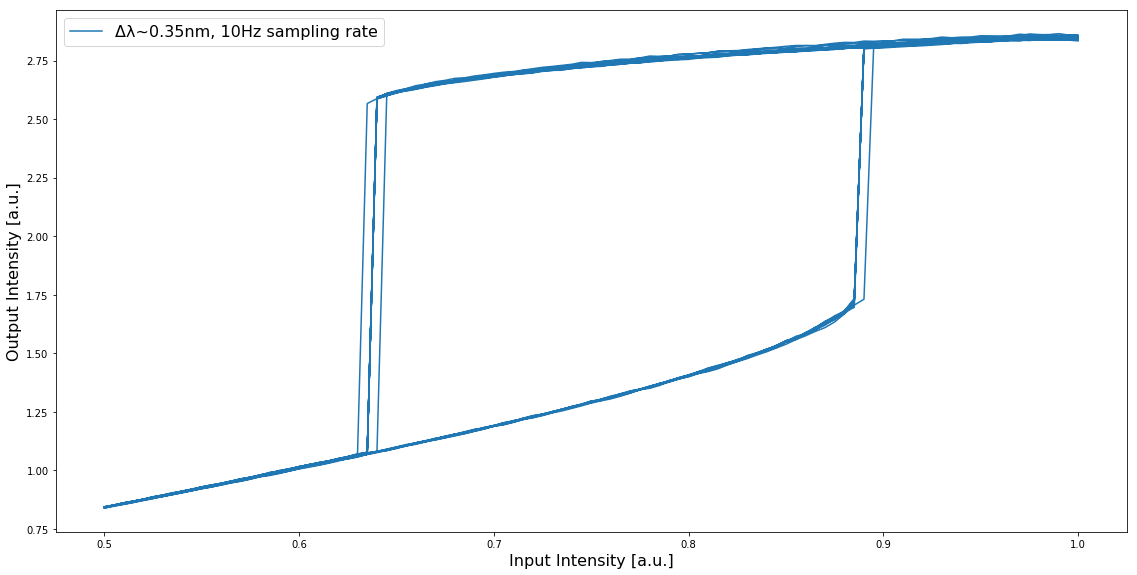
\includegraphics[draft,width=9cm,height=6cm]{figures/foo.png}
	\caption{image/scheme of the minimatrix}
	\label{fig:minimatrix_full}
\end{figure}

\section{Setup}

\section{Characterization of the Activation Function}
\label{sec:Characterization_of_the_Activation_Function}
Characterization of the activation function

\section{Test of a Trained ANN}
\label{sec:Test_of_a_Trained ANN}
Test of the activation function

% conclusive chapter ~ 5pg
\chapter*{Conclusion}
\markboth{CONCLUSION}{}
\addcontentsline{toc}{chapter}{Conclusions}

% total ~ 60pg

% Bibliography
%\cleardoublepage
\printbibliography[heading=bibintoc]%,title={References}]

% Aknowledgements
\chapter*{Aknowledgements}
\markboth{AKNOWLEDGEMENTS}{}
\addcontentsline{toc}{chapter}{Aknowledgements}

\end{document}